\documentclass[twoside]{book}

% Packages required by doxygen
\usepackage{fixltx2e}
\usepackage{calc}
\usepackage{doxygen}
\usepackage[export]{adjustbox} % also loads graphicx
\usepackage{graphicx}
\usepackage[utf8]{inputenc}
\usepackage{makeidx}
\usepackage{multicol}
\usepackage{multirow}
\PassOptionsToPackage{warn}{textcomp}
\usepackage{textcomp}
\usepackage[nointegrals]{wasysym}
\usepackage[table]{xcolor}

% Font selection
\usepackage[T1]{fontenc}
\usepackage[scaled=.90]{helvet}
\usepackage{courier}
\usepackage{amssymb}
\usepackage{sectsty}
\renewcommand{\familydefault}{\sfdefault}
\allsectionsfont{%
  \fontseries{bc}\selectfont%
  \color{darkgray}%
}
\renewcommand{\DoxyLabelFont}{%
  \fontseries{bc}\selectfont%
  \color{darkgray}%
}
\newcommand{\+}{\discretionary{\mbox{\scriptsize$\hookleftarrow$}}{}{}}

% Page & text layout
\usepackage{geometry}
\geometry{%
  a4paper,%
  top=2.5cm,%
  bottom=2.5cm,%
  left=2.5cm,%
  right=2.5cm%
}
\tolerance=750
\hfuzz=15pt
\hbadness=750
\setlength{\emergencystretch}{15pt}
\setlength{\parindent}{0cm}
\setlength{\parskip}{3ex plus 2ex minus 2ex}
\makeatletter
\renewcommand{\paragraph}{%
  \@startsection{paragraph}{4}{0ex}{-1.0ex}{1.0ex}{%
    \normalfont\normalsize\bfseries\SS@parafont%
  }%
}
\renewcommand{\subparagraph}{%
  \@startsection{subparagraph}{5}{0ex}{-1.0ex}{1.0ex}{%
    \normalfont\normalsize\bfseries\SS@subparafont%
  }%
}
\makeatother

% Headers & footers
\usepackage{fancyhdr}
\pagestyle{fancyplain}
\fancyhead[LE]{\fancyplain{}{\bfseries\thepage}}
\fancyhead[CE]{\fancyplain{}{}}
\fancyhead[RE]{\fancyplain{}{\bfseries\leftmark}}
\fancyhead[LO]{\fancyplain{}{\bfseries\rightmark}}
\fancyhead[CO]{\fancyplain{}{}}
\fancyhead[RO]{\fancyplain{}{\bfseries\thepage}}
\fancyfoot[LE]{\fancyplain{}{}}
\fancyfoot[CE]{\fancyplain{}{}}
\fancyfoot[RE]{\fancyplain{}{\bfseries\scriptsize Generated by Doxygen }}
\fancyfoot[LO]{\fancyplain{}{\bfseries\scriptsize Generated by Doxygen }}
\fancyfoot[CO]{\fancyplain{}{}}
\fancyfoot[RO]{\fancyplain{}{}}
\renewcommand{\footrulewidth}{0.4pt}
\renewcommand{\chaptermark}[1]{%
  \markboth{#1}{}%
}
\renewcommand{\sectionmark}[1]{%
  \markright{\thesection\ #1}%
}

% Indices & bibliography
\usepackage{natbib}
\usepackage[titles]{tocloft}
\setcounter{tocdepth}{3}
\setcounter{secnumdepth}{5}
\makeindex

% Hyperlinks (required, but should be loaded last)
\usepackage{ifpdf}
\ifpdf
  \usepackage[pdftex,pagebackref=true]{hyperref}
\else
  \usepackage[ps2pdf,pagebackref=true]{hyperref}
\fi
\hypersetup{%
  colorlinks=true,%
  linkcolor=blue,%
  citecolor=blue,%
  unicode%
}

% Custom commands
\newcommand{\clearemptydoublepage}{%
  \newpage{\pagestyle{empty}\cleardoublepage}%
}

\usepackage{caption}
\captionsetup{labelsep=space,justification=centering,font={bf},singlelinecheck=off,skip=4pt,position=top}

%===== C O N T E N T S =====

\begin{document}

% Titlepage & ToC
\hypersetup{pageanchor=false,
             bookmarksnumbered=true,
             pdfencoding=unicode
            }
\pagenumbering{alph}
\begin{titlepage}
\vspace*{7cm}
\begin{center}%
{\Large Timescaled DB }\\
\vspace*{1cm}
{\large Generated by Doxygen 1.8.13}\\
\end{center}
\end{titlepage}
\clearemptydoublepage
\pagenumbering{roman}
\tableofcontents
\clearemptydoublepage
\pagenumbering{arabic}
\hypersetup{pageanchor=true}

%--- Begin generated contents ---
\chapter{Timescaledb}
\label{index}\hypertarget{index}{}\subsection*{Timescaledb provides importing csv file, sorting by timestamp (fresh data goes first) and writing sorted data to database along with response by H\+T\+ML table of sorted data.}

Author\+: {\bfseries Cherniaev Egor} \# To perfom all functions properly, user should have following informations


\begin{DoxyEnumerate}
\item Path to csv file
\item Number of column were timestamp is presented
\item Database connection data(\href{https://www.postgresql.org/docs/10/libpq-connect.html}{\tt {\ttfamily connetion string}}). Example {\ttfamily \char`\"{}host=localhost dbname=your\+\_\+database user=your\+\_\+user password=your\+\_\+password\char`\"{}}. Only this information is used to connect database.
\item Table name
\end{DoxyEnumerate}

After data has correctly been supplied, work begins. In other cases, an error occurs and error description is returned (more on that later).

\subsection*{Requirements (for server)}


\begin{DoxyItemize}
\item \href{https://kore.io/}{\tt Kore.\+io framework}
\item \href{https://www.postgresql.org/}{\tt Postgresql}
\end{DoxyItemize}

\subsection*{How to use?}

To {\bfseries run kore application} use {\ttfamily kodev clean \&\& kodev build \&\& kodev run} inside of main directory

Then, all you need is to collect all needed information and then perform G\+ET H\+T\+TP request.

{\bfseries Collect \+:} path/to/file.\+csv, my\+\_\+column\+\_\+with\+\_\+timestamp, my\+\_\+table\+\_\+name.

{\bfseries Do \+:}{\ttfamily \href{http://host_server:port/?pth=path%2Fto%2Ffile.csv&ts=my_column_with_timestamp&tbl=my_table_name}{\tt http\+://host\+\_\+server\+:port/?pth=path\%2\+Fto\%2\+Ffile.\+csv\&ts=my\+\_\+column\+\_\+with\+\_\+timestamp\&tbl=my\+\_\+table\+\_\+name}}

Request should contain following query {\bfseries parameters}\+:
\begin{DoxyItemize}
\item {\bfseries pth} -\/ path to file to perform sorting on,file should exist
\item {\bfseries ts} -\/ timestamp column number, wich is used to identify timestamp({\bfseries column are counted from 0})
\item {\bfseries tbl} -\/ table name.
\end{DoxyItemize}

All with U\+RL encoding. If the table doesn\textquotesingle{}t exist -\/ {\itshape it will be created} with the name you have used. After the request was received, a sorting process begins. In case of fail, an error report is returned and the user may try to change some supplied information. General errors are described below. In this version it is impossible to change the database connection string without code changing or to change timestamp format. All types of timestamp are available. The only restriction is-\/ they should follow \href{https://en.wikipedia.org/wiki/ISO_8601}{\tt I\+SO 8601} to perform sorting correctly. If the file is \char`\"{}broken\char`\"{}, some unexpected errors may occur.

\subsection*{General activity description}

The file gets loaded and timestamps are found. Then goes sorting. Sorting uses \href{https://en.wikipedia.org/wiki/Comb_sort}{\tt the combo sort algorithm}. After sorting, timestamps are ordered this way\+: {\bfseries fresh data first} (before 2001 2004 1900 2017 ---$>$ after 2017 2004 2001 1900). As it has been finished, database query is built and performed. In case of success, the H\+T\+ML table is built and the program will send it as the response.

\subsection*{Possible errors (errors explanation)}

{\ttfamily \+\_\+\+The response could not be created correctly\+\_\+} \+: Means that an internal error happened. Try again or check csv file you are working with.

{\ttfamily \+\_\+\+Error in querying S\+Q\+L\+\_\+} \+: Means that connection to database for some reasons was not accepted. Check connection string or your rights related to this database

{\ttfamily \+\_\+\+Error in creating table\+\_\+} \+: Table from file could not be created(header in file or data in file are not acceptable for database)

{\ttfamily \+\_\+\+Error while sorting C\+S\+V(check file or parameters)\+\_\+}\+: The most common and possible error. Means that file contains error in format or that you have entered wrong timestamp column number. What is considered as error? First of all -\/ if file does not exist. Then -\/ timestamps have different length, lines have different number of columns(it does not match header). \char`\"{}\+Broken files\char`\"{} this cause error too.

{\ttfamily \+\_\+\+Error in parameters\+\_\+} \+: Wrong identifiers used(pth--$>$path--$>$error) and/or data does not fit filter(e.\+i. ts-\/timestamp column number-\/ contains anything else but decimal number). Some additional info could be returned, to expand error.

\begin{quote}
{\bfseries C\+H\+E\+CK B\+E\+F\+O\+RE U\+SE}\+: timestamp\+\_\+col(http\+:ts), path\+\_\+to\+\_\+csv(http\+:pth). F\+OR D\+A\+T\+A\+B\+A\+SE \+: table\+\_\+name(http\+:tbl), max\+\_\+entry\+\_\+size(in code)\end{quote}

\chapter{File Index}
\section{File List}
Here is a list of all files with brief descriptions\+:\begin{DoxyCompactList}
\item\contentsline{section}{src/\hyperlink{agrlib__v1_8h}{agrlib\+\_\+v1.\+h} }{\pageref{agrlib__v1_8h}}{}
\item\contentsline{section}{src/\hyperlink{agrlib__v2_8h}{agrlib\+\_\+v2.\+h} }{\pageref{agrlib__v2_8h}}{}
\item\contentsline{section}{src/\hyperlink{core_8c}{core.\+c} }{\pageref{core_8c}}{}
\end{DoxyCompactList}

\chapter{File Documentation}
\hypertarget{agrlib__v1_8h}{}\section{src/agrlib\+\_\+v1.h File Reference}
\label{agrlib__v1_8h}\index{src/agrlib\+\_\+v1.\+h@{src/agrlib\+\_\+v1.\+h}}
{\ttfamily \#include $<$stdio.\+h$>$}\newline
{\ttfamily \#include $<$stdlib.\+h$>$}\newline
Include dependency graph for agrlib\+\_\+v1.\+h\+:\nopagebreak
\begin{figure}[H]
\begin{center}
\leavevmode
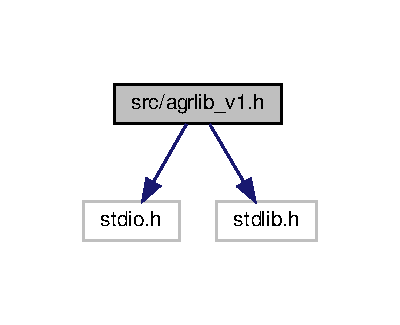
\includegraphics[width=192pt]{agrlib__v1_8h__incl}
\end{center}
\end{figure}
\subsection*{Macros}
\begin{DoxyCompactItemize}
\item 
\#define \hyperlink{agrlib__v1_8h_a5ab5b9aaf3850b085ca39abf901b2751}{T\+E\+S\+T\+\_\+\+C\+A\+SE}
\end{DoxyCompactItemize}
\subsection*{Functions}
\begin{DoxyCompactItemize}
\item 
int \hyperlink{agrlib__v1_8h_a0307984afb426de0d910e5fc8eb5af27}{csv\+\_\+import} (char \hyperlink{core_8c_a4b2ae53d82dc2d82a6ba3d6488e3638f}{path\+\_\+to\+\_\+csv}\mbox{[}$\,$\mbox{]})
\begin{DoxyCompactList}\small\item\em Function perform import of file.\+Input value\+: path to file. Return value\+: D\+O\+NE or E\+R\+R\+OR. \end{DoxyCompactList}\item 
int \hyperlink{agrlib__v1_8h_a7a14e18fe42a95fdce291f1ffd1be5c2}{csv\+\_\+info} (char $\ast$\hyperlink{agrlib__v1_8h_ab00f83b047d06986d6709f8ac535b192}{csv})
\item 
int \hyperlink{agrlib__v1_8h_a605396290960b729c55527ce1168deda}{init\+\_\+memory} (size\+\_\+t len, int case\+\_\+)
\item 
int \hyperlink{agrlib__v1_8h_aebc31f51013d2dc2c24e280b63e35c3f}{csv\+\_\+get\+\_\+lines} (char $\ast$\hyperlink{agrlib__v1_8h_ab00f83b047d06986d6709f8ac535b192}{csv})
\item 
int \hyperlink{agrlib__v1_8h_aadd713f59dccacdf303f1eae5ff3cbbe}{csv\+\_\+get\+\_\+timestamps} (char $\ast$\hyperlink{agrlib__v1_8h_ab00f83b047d06986d6709f8ac535b192}{csv})
\item 
int \hyperlink{agrlib__v1_8h_a21172191aa50a1ec76d88e728f9c69d4}{sort\+\_\+timepointers} (char $\ast$$\ast$time, char $\ast$$\ast$line)
\item 
int \hyperlink{agrlib__v1_8h_ab91f89f6a19d310763428e1bf599f4fe}{compare\+\_\+timestamps} (char $\ast$first, char $\ast$second)
\item 
size\+\_\+t \hyperlink{agrlib__v1_8h_ad9931ba3f9b842cdf853e586e986ab50}{new\+\_\+gap} (size\+\_\+t gap)
\item 
char $\ast$$\ast$$\ast$ \hyperlink{agrlib__v1_8h_af68635331d12bfd02f30d9b4be320cfa}{agregate} (char \hyperlink{core_8c_a4b2ae53d82dc2d82a6ba3d6488e3638f}{path\+\_\+to\+\_\+csv}\mbox{[}$\,$\mbox{]})
\item 
void \hyperlink{agrlib__v1_8h_a19ca95ef173bf8ed186fd3c4d0aede1f}{show\+\_\+hiden\+\_\+time} (char $\ast$timestamp)
\item 
void \hyperlink{agrlib__v1_8h_a4df9c8a3fc1c3470cdc57ecfb548fd95}{show\+\_\+hiden\+\_\+string} (char $\ast$line)
\item 
void \hyperlink{agrlib__v1_8h_a93d82a5a51eb0de86f629e86dce96202}{general\+\_\+check} (int case\+\_\+)
\end{DoxyCompactItemize}
\subsection*{Variables}
\begin{DoxyCompactItemize}
\item 
char \hyperlink{agrlib__v1_8h_a2f44b091be60ccdd664997eb163d2ff4}{sep} = \textquotesingle{},\textquotesingle{}
\item 
int \hyperlink{agrlib__v1_8h_a4409b51f47ad8c26d98b227bf26bfbd9}{end\+\_\+\+CR} = 0x0D
\item 
int \hyperlink{agrlib__v1_8h_abb7d175ad428e618e66b9d002a475cf2}{end\+\_\+\+LF} = 0x0A
\item 
size\+\_\+t \hyperlink{agrlib__v1_8h_adfdc908b893f72ef73c8850671ba538f}{timestamp\+\_\+col} = 9
\item 
int \hyperlink{agrlib__v1_8h_aeed51c87c57a3eb984514da8000aeb7b}{timestamp\+\_\+len} = 10
\item 
int \hyperlink{agrlib__v1_8h_a8466c885b251cd7cfa286745837b5347}{max\+\_\+try} = 5
\item 
F\+I\+LE $\ast$ \hyperlink{agrlib__v1_8h_a82500a31718a0b612f28d06d2a448e04}{input\+\_\+csv}
\item 
char $\ast$ \hyperlink{agrlib__v1_8h_ab00f83b047d06986d6709f8ac535b192}{csv} = N\+U\+LL
\item 
char $\ast$ \hyperlink{agrlib__v1_8h_a23e167da0fef4284e753ab3fb1b7b4e6}{csv\+\_\+end} = N\+U\+LL
\item 
size\+\_\+t \hyperlink{agrlib__v1_8h_aacf1d5147428082c66dcc6f0bce5e134}{max\+\_\+line\+\_\+len} = 0
\end{DoxyCompactItemize}


\subsection{Macro Definition Documentation}
\mbox{\Hypertarget{agrlib__v1_8h_a5ab5b9aaf3850b085ca39abf901b2751}\label{agrlib__v1_8h_a5ab5b9aaf3850b085ca39abf901b2751}} 
\index{agrlib\+\_\+v1.\+h@{agrlib\+\_\+v1.\+h}!T\+E\+S\+T\+\_\+\+C\+A\+SE@{T\+E\+S\+T\+\_\+\+C\+A\+SE}}
\index{T\+E\+S\+T\+\_\+\+C\+A\+SE@{T\+E\+S\+T\+\_\+\+C\+A\+SE}!agrlib\+\_\+v1.\+h@{agrlib\+\_\+v1.\+h}}
\subsubsection{\texorpdfstring{T\+E\+S\+T\+\_\+\+C\+A\+SE}{TEST\_CASE}}
{\footnotesize\ttfamily \#define T\+E\+S\+T\+\_\+\+C\+A\+SE}



\subsection{Function Documentation}
\mbox{\Hypertarget{agrlib__v1_8h_af68635331d12bfd02f30d9b4be320cfa}\label{agrlib__v1_8h_af68635331d12bfd02f30d9b4be320cfa}} 
\index{agrlib\+\_\+v1.\+h@{agrlib\+\_\+v1.\+h}!agregate@{agregate}}
\index{agregate@{agregate}!agrlib\+\_\+v1.\+h@{agrlib\+\_\+v1.\+h}}
\subsubsection{\texorpdfstring{agregate()}{agregate()}}
{\footnotesize\ttfamily char $\ast$$\ast$$\ast$ agregate (\begin{DoxyParamCaption}\item[{char}]{path\+\_\+to\+\_\+csv\mbox{[}$\,$\mbox{]} }\end{DoxyParamCaption})}

\mbox{\Hypertarget{agrlib__v1_8h_ab91f89f6a19d310763428e1bf599f4fe}\label{agrlib__v1_8h_ab91f89f6a19d310763428e1bf599f4fe}} 
\index{agrlib\+\_\+v1.\+h@{agrlib\+\_\+v1.\+h}!compare\+\_\+timestamps@{compare\+\_\+timestamps}}
\index{compare\+\_\+timestamps@{compare\+\_\+timestamps}!agrlib\+\_\+v1.\+h@{agrlib\+\_\+v1.\+h}}
\subsubsection{\texorpdfstring{compare\+\_\+timestamps()}{compare\_timestamps()}}
{\footnotesize\ttfamily int compare\+\_\+timestamps (\begin{DoxyParamCaption}\item[{char $\ast$}]{first,  }\item[{char $\ast$}]{second }\end{DoxyParamCaption})}

Comparison is done by subtraction and comparison with zero, so it is important to follow timestamps format Return value 1 if first(passed value) $>$ second (passed value) 2 if first $<$ second 3 if first = second In T\+E\+S\+T\+\_\+\+C\+A\+SE some additional information is shown

Comparing we loop through timestamps subtracting values Return values reflects relations between First and Second values \mbox{\Hypertarget{agrlib__v1_8h_aebc31f51013d2dc2c24e280b63e35c3f}\label{agrlib__v1_8h_aebc31f51013d2dc2c24e280b63e35c3f}} 
\index{agrlib\+\_\+v1.\+h@{agrlib\+\_\+v1.\+h}!csv\+\_\+get\+\_\+lines@{csv\+\_\+get\+\_\+lines}}
\index{csv\+\_\+get\+\_\+lines@{csv\+\_\+get\+\_\+lines}!agrlib\+\_\+v1.\+h@{agrlib\+\_\+v1.\+h}}
\subsubsection{\texorpdfstring{csv\+\_\+get\+\_\+lines()}{csv\_get\_lines()}}
{\footnotesize\ttfamily int csv\+\_\+get\+\_\+lines (\begin{DoxyParamCaption}\item[{char $\ast$}]{csv }\end{DoxyParamCaption})}

Getting lines beginnings starts with memory allocation. We need memory for pointers array with length equal to the number of rows

In case of fail we will try up try max try number

Then we search for position of each first not null symbol and save reference on it \mbox{\Hypertarget{agrlib__v1_8h_aadd713f59dccacdf303f1eae5ff3cbbe}\label{agrlib__v1_8h_aadd713f59dccacdf303f1eae5ff3cbbe}} 
\index{agrlib\+\_\+v1.\+h@{agrlib\+\_\+v1.\+h}!csv\+\_\+get\+\_\+timestamps@{csv\+\_\+get\+\_\+timestamps}}
\index{csv\+\_\+get\+\_\+timestamps@{csv\+\_\+get\+\_\+timestamps}!agrlib\+\_\+v1.\+h@{agrlib\+\_\+v1.\+h}}
\subsubsection{\texorpdfstring{csv\+\_\+get\+\_\+timestamps()}{csv\_get\_timestamps()}}
{\footnotesize\ttfamily int csv\+\_\+get\+\_\+timestamps (\begin{DoxyParamCaption}\item[{char $\ast$}]{csv }\end{DoxyParamCaption})}

Getting timestamps pointers for further comparison start with memory a allocation. We try to allocate memory as well several times

To indicate if current position in file contains timestamp or not we will count columns If file contains an error and we exceed the number of columns -\/work stops.

As timestamp is found and its first character address is stored -\/ we do not expect timestamps in this line any more

All timestamps should be the same length, which is never exceeded during timestamps comparison

Header does not take part in counting, so first -\/ we must pass it

To avoid errors in column number we indicate step from meaningful part to meaning less If at this moments we did not met enough separators -\/ error

Each symbol is checked for separator or E\+OL

E\+OL means that we are in useless part

If timestamp is located at the end of line -\/ its length is counted here.

As well at the end of line we check for number of columns to be the same as counted in header

Another error is reaching end of line and without reaching timestamp column.

Indication of non header line is \+: timestamp length counting has started, but header\+\_\+passed is still false .

Next error is different length of timestamps, which means that error if no timestamp found. If something else is in column of ts, but of the same length -\/ it ok, as well it will be sorted.

Length of timestamp is as well controlled/counted when separator is met.

Finally -\/ an address of first symbol in timestamps columns is taken. \mbox{\Hypertarget{agrlib__v1_8h_a0307984afb426de0d910e5fc8eb5af27}\label{agrlib__v1_8h_a0307984afb426de0d910e5fc8eb5af27}} 
\index{agrlib\+\_\+v1.\+h@{agrlib\+\_\+v1.\+h}!csv\+\_\+import@{csv\+\_\+import}}
\index{csv\+\_\+import@{csv\+\_\+import}!agrlib\+\_\+v1.\+h@{agrlib\+\_\+v1.\+h}}
\subsubsection{\texorpdfstring{csv\+\_\+import()}{csv\_import()}}
{\footnotesize\ttfamily int csv\+\_\+import (\begin{DoxyParamCaption}\item[{char}]{path\+\_\+to\+\_\+csv\mbox{[}$\,$\mbox{]} }\end{DoxyParamCaption})}



Function perform import of file.\+Input value\+: path to file. Return value\+: D\+O\+NE or E\+R\+R\+OR. 

\mbox{\Hypertarget{agrlib__v1_8h_a7a14e18fe42a95fdce291f1ffd1be5c2}\label{agrlib__v1_8h_a7a14e18fe42a95fdce291f1ffd1be5c2}} 
\index{agrlib\+\_\+v1.\+h@{agrlib\+\_\+v1.\+h}!csv\+\_\+info@{csv\+\_\+info}}
\index{csv\+\_\+info@{csv\+\_\+info}!agrlib\+\_\+v1.\+h@{agrlib\+\_\+v1.\+h}}
\subsubsection{\texorpdfstring{csv\+\_\+info()}{csv\_info()}}
{\footnotesize\ttfamily int csv\+\_\+info (\begin{DoxyParamCaption}\item[{char $\ast$}]{csv }\end{DoxyParamCaption})}

First,lets count columns. For this we use first line, as it is considered to be header

So, each character is compared with separator or E\+OL

Each found separator increase column number

As the E\+OL reached -\/ we increase column number again \+: ... , ... , ... has 3 col, but only 2 separators

Here we will also check if file contains more than one line.

If only one line found -\/ we return, as it has no reason to continue sorting

Next -\/ count meaningful lines and maximum line length. From here line becomes sequence of characters delimited by \textquotesingle{}\textbackslash{}0\textquotesingle{} (max\+\_\+len -\/ maximum length, cur\+\_\+len -\/ current length)

Replacing all E\+OL with \textquotesingle{}\textbackslash{}0\textquotesingle{} will make searching easier

In test case, information about file will be printed \mbox{\Hypertarget{agrlib__v1_8h_a93d82a5a51eb0de86f629e86dce96202}\label{agrlib__v1_8h_a93d82a5a51eb0de86f629e86dce96202}} 
\index{agrlib\+\_\+v1.\+h@{agrlib\+\_\+v1.\+h}!general\+\_\+check@{general\+\_\+check}}
\index{general\+\_\+check@{general\+\_\+check}!agrlib\+\_\+v1.\+h@{agrlib\+\_\+v1.\+h}}
\subsubsection{\texorpdfstring{general\+\_\+check()}{general\_check()}}
{\footnotesize\ttfamily void general\+\_\+check (\begin{DoxyParamCaption}\item[{int}]{case\+\_\+ }\end{DoxyParamCaption})}

Shows all timestamps(1), saved by pointers or lines(2), saved by pointers \mbox{\Hypertarget{agrlib__v1_8h_a605396290960b729c55527ce1168deda}\label{agrlib__v1_8h_a605396290960b729c55527ce1168deda}} 
\index{agrlib\+\_\+v1.\+h@{agrlib\+\_\+v1.\+h}!init\+\_\+memory@{init\+\_\+memory}}
\index{init\+\_\+memory@{init\+\_\+memory}!agrlib\+\_\+v1.\+h@{agrlib\+\_\+v1.\+h}}
\subsubsection{\texorpdfstring{init\+\_\+memory()}{init\_memory()}}
{\footnotesize\ttfamily int init\+\_\+memory (\begin{DoxyParamCaption}\item[{size\+\_\+t}]{len,  }\item[{int}]{case\+\_\+ }\end{DoxyParamCaption})}

For better structure some memory initialization is located here. Global pointers timestamp and lines getting memory from here. Input\+: len -\/ size of memory to allocate, case\+\_\+ -\/ for which pointer(1,2,3) \mbox{\Hypertarget{agrlib__v1_8h_ad9931ba3f9b842cdf853e586e986ab50}\label{agrlib__v1_8h_ad9931ba3f9b842cdf853e586e986ab50}} 
\index{agrlib\+\_\+v1.\+h@{agrlib\+\_\+v1.\+h}!new\+\_\+gap@{new\+\_\+gap}}
\index{new\+\_\+gap@{new\+\_\+gap}!agrlib\+\_\+v1.\+h@{agrlib\+\_\+v1.\+h}}
\subsubsection{\texorpdfstring{new\+\_\+gap()}{new\_gap()}}
{\footnotesize\ttfamily size\+\_\+t new\+\_\+gap (\begin{DoxyParamCaption}\item[{size\+\_\+t}]{gap }\end{DoxyParamCaption})}

New gap for sorting is formed from rows number and after first loop of algorithm from last gap. Conditions of gap formation could be changed \mbox{\Hypertarget{agrlib__v1_8h_a4df9c8a3fc1c3470cdc57ecfb548fd95}\label{agrlib__v1_8h_a4df9c8a3fc1c3470cdc57ecfb548fd95}} 
\index{agrlib\+\_\+v1.\+h@{agrlib\+\_\+v1.\+h}!show\+\_\+hiden\+\_\+string@{show\+\_\+hiden\+\_\+string}}
\index{show\+\_\+hiden\+\_\+string@{show\+\_\+hiden\+\_\+string}!agrlib\+\_\+v1.\+h@{agrlib\+\_\+v1.\+h}}
\subsubsection{\texorpdfstring{show\+\_\+hiden\+\_\+string()}{show\_hiden\_string()}}
{\footnotesize\ttfamily void show\+\_\+hiden\+\_\+string (\begin{DoxyParamCaption}\item[{char $\ast$}]{line }\end{DoxyParamCaption})}

Helpful when testing. Show line by its pointer \mbox{\Hypertarget{agrlib__v1_8h_a19ca95ef173bf8ed186fd3c4d0aede1f}\label{agrlib__v1_8h_a19ca95ef173bf8ed186fd3c4d0aede1f}} 
\index{agrlib\+\_\+v1.\+h@{agrlib\+\_\+v1.\+h}!show\+\_\+hiden\+\_\+time@{show\+\_\+hiden\+\_\+time}}
\index{show\+\_\+hiden\+\_\+time@{show\+\_\+hiden\+\_\+time}!agrlib\+\_\+v1.\+h@{agrlib\+\_\+v1.\+h}}
\subsubsection{\texorpdfstring{show\+\_\+hiden\+\_\+time()}{show\_hiden\_time()}}
{\footnotesize\ttfamily void show\+\_\+hiden\+\_\+time (\begin{DoxyParamCaption}\item[{char $\ast$}]{timestamp }\end{DoxyParamCaption})}

Helpful when testing. Show timestamps by pointer \mbox{\Hypertarget{agrlib__v1_8h_a21172191aa50a1ec76d88e728f9c69d4}\label{agrlib__v1_8h_a21172191aa50a1ec76d88e728f9c69d4}} 
\index{agrlib\+\_\+v1.\+h@{agrlib\+\_\+v1.\+h}!sort\+\_\+timepointers@{sort\+\_\+timepointers}}
\index{sort\+\_\+timepointers@{sort\+\_\+timepointers}!agrlib\+\_\+v1.\+h@{agrlib\+\_\+v1.\+h}}
\subsubsection{\texorpdfstring{sort\+\_\+timepointers()}{sort\_timepointers()}}
{\footnotesize\ttfamily int sort\+\_\+timepointers (\begin{DoxyParamCaption}\item[{char $\ast$$\ast$}]{time,  }\item[{char $\ast$$\ast$}]{line }\end{DoxyParamCaption})}

Algorithm is based on bubble sort. The only difference is in shrinking gap between two compared values. At last stages it becomes pure bubble sort.

Before comparison we would check if it worth to be done -\/ if csv has only 2 rows it has no meaning.

In other case, first thing to do -\/ step over header.

Then define some temporary holders for compared objects We compare timestamps but the line order gets changed too

Sorting loop starts with getting new gap

Then we compare two timestamps with compare\+\_\+timestamps function. IF Y\+OU N\+E\+ED TO C\+H\+A\+N\+GE O\+R\+D\+ER -\/ S\+ET 2 I\+N\+S\+T\+E\+AD OF 1 IN IF C\+O\+N\+D\+I\+T\+I\+ON If the order is ok, go on, else -\/ swap the pointers 

\subsection{Variable Documentation}
\mbox{\Hypertarget{agrlib__v1_8h_ab00f83b047d06986d6709f8ac535b192}\label{agrlib__v1_8h_ab00f83b047d06986d6709f8ac535b192}} 
\index{agrlib\+\_\+v1.\+h@{agrlib\+\_\+v1.\+h}!csv@{csv}}
\index{csv@{csv}!agrlib\+\_\+v1.\+h@{agrlib\+\_\+v1.\+h}}
\subsubsection{\texorpdfstring{csv}{csv}}
{\footnotesize\ttfamily char$\ast$ csv = N\+U\+LL}

\mbox{\Hypertarget{agrlib__v1_8h_a23e167da0fef4284e753ab3fb1b7b4e6}\label{agrlib__v1_8h_a23e167da0fef4284e753ab3fb1b7b4e6}} 
\index{agrlib\+\_\+v1.\+h@{agrlib\+\_\+v1.\+h}!csv\+\_\+end@{csv\+\_\+end}}
\index{csv\+\_\+end@{csv\+\_\+end}!agrlib\+\_\+v1.\+h@{agrlib\+\_\+v1.\+h}}
\subsubsection{\texorpdfstring{csv\+\_\+end}{csv\_end}}
{\footnotesize\ttfamily char$\ast$ csv\+\_\+end = N\+U\+LL}

\mbox{\Hypertarget{agrlib__v1_8h_a4409b51f47ad8c26d98b227bf26bfbd9}\label{agrlib__v1_8h_a4409b51f47ad8c26d98b227bf26bfbd9}} 
\index{agrlib\+\_\+v1.\+h@{agrlib\+\_\+v1.\+h}!end\+\_\+\+CR@{end\+\_\+\+CR}}
\index{end\+\_\+\+CR@{end\+\_\+\+CR}!agrlib\+\_\+v1.\+h@{agrlib\+\_\+v1.\+h}}
\subsubsection{\texorpdfstring{end\+\_\+\+CR}{end\_CR}}
{\footnotesize\ttfamily int end\+\_\+\+CR = 0x0D}

\mbox{\Hypertarget{agrlib__v1_8h_abb7d175ad428e618e66b9d002a475cf2}\label{agrlib__v1_8h_abb7d175ad428e618e66b9d002a475cf2}} 
\index{agrlib\+\_\+v1.\+h@{agrlib\+\_\+v1.\+h}!end\+\_\+\+LF@{end\+\_\+\+LF}}
\index{end\+\_\+\+LF@{end\+\_\+\+LF}!agrlib\+\_\+v1.\+h@{agrlib\+\_\+v1.\+h}}
\subsubsection{\texorpdfstring{end\+\_\+\+LF}{end\_LF}}
{\footnotesize\ttfamily int end\+\_\+\+LF = 0x0A}

\mbox{\Hypertarget{agrlib__v1_8h_a82500a31718a0b612f28d06d2a448e04}\label{agrlib__v1_8h_a82500a31718a0b612f28d06d2a448e04}} 
\index{agrlib\+\_\+v1.\+h@{agrlib\+\_\+v1.\+h}!input\+\_\+csv@{input\+\_\+csv}}
\index{input\+\_\+csv@{input\+\_\+csv}!agrlib\+\_\+v1.\+h@{agrlib\+\_\+v1.\+h}}
\subsubsection{\texorpdfstring{input\+\_\+csv}{input\_csv}}
{\footnotesize\ttfamily F\+I\+LE$\ast$ input\+\_\+csv}

\mbox{\Hypertarget{agrlib__v1_8h_aacf1d5147428082c66dcc6f0bce5e134}\label{agrlib__v1_8h_aacf1d5147428082c66dcc6f0bce5e134}} 
\index{agrlib\+\_\+v1.\+h@{agrlib\+\_\+v1.\+h}!max\+\_\+line\+\_\+len@{max\+\_\+line\+\_\+len}}
\index{max\+\_\+line\+\_\+len@{max\+\_\+line\+\_\+len}!agrlib\+\_\+v1.\+h@{agrlib\+\_\+v1.\+h}}
\subsubsection{\texorpdfstring{max\+\_\+line\+\_\+len}{max\_line\_len}}
{\footnotesize\ttfamily size\+\_\+t max\+\_\+line\+\_\+len = 0}

\mbox{\Hypertarget{agrlib__v1_8h_a8466c885b251cd7cfa286745837b5347}\label{agrlib__v1_8h_a8466c885b251cd7cfa286745837b5347}} 
\index{agrlib\+\_\+v1.\+h@{agrlib\+\_\+v1.\+h}!max\+\_\+try@{max\+\_\+try}}
\index{max\+\_\+try@{max\+\_\+try}!agrlib\+\_\+v1.\+h@{agrlib\+\_\+v1.\+h}}
\subsubsection{\texorpdfstring{max\+\_\+try}{max\_try}}
{\footnotesize\ttfamily int max\+\_\+try = 5}

\mbox{\Hypertarget{agrlib__v1_8h_a2f44b091be60ccdd664997eb163d2ff4}\label{agrlib__v1_8h_a2f44b091be60ccdd664997eb163d2ff4}} 
\index{agrlib\+\_\+v1.\+h@{agrlib\+\_\+v1.\+h}!sep@{sep}}
\index{sep@{sep}!agrlib\+\_\+v1.\+h@{agrlib\+\_\+v1.\+h}}
\subsubsection{\texorpdfstring{sep}{sep}}
{\footnotesize\ttfamily char sep = \textquotesingle{},\textquotesingle{}}

\mbox{\Hypertarget{agrlib__v1_8h_adfdc908b893f72ef73c8850671ba538f}\label{agrlib__v1_8h_adfdc908b893f72ef73c8850671ba538f}} 
\index{agrlib\+\_\+v1.\+h@{agrlib\+\_\+v1.\+h}!timestamp\+\_\+col@{timestamp\+\_\+col}}
\index{timestamp\+\_\+col@{timestamp\+\_\+col}!agrlib\+\_\+v1.\+h@{agrlib\+\_\+v1.\+h}}
\subsubsection{\texorpdfstring{timestamp\+\_\+col}{timestamp\_col}}
{\footnotesize\ttfamily size\+\_\+t timestamp\+\_\+col = 9}

\mbox{\Hypertarget{agrlib__v1_8h_aeed51c87c57a3eb984514da8000aeb7b}\label{agrlib__v1_8h_aeed51c87c57a3eb984514da8000aeb7b}} 
\index{agrlib\+\_\+v1.\+h@{agrlib\+\_\+v1.\+h}!timestamp\+\_\+len@{timestamp\+\_\+len}}
\index{timestamp\+\_\+len@{timestamp\+\_\+len}!agrlib\+\_\+v1.\+h@{agrlib\+\_\+v1.\+h}}
\subsubsection{\texorpdfstring{timestamp\+\_\+len}{timestamp\_len}}
{\footnotesize\ttfamily int timestamp\+\_\+len = 10}


\hypertarget{agrlib__v2_8h}{}\section{src/agrlib\+\_\+v2.h File Reference}
\label{agrlib__v2_8h}\index{src/agrlib\+\_\+v2.\+h@{src/agrlib\+\_\+v2.\+h}}
{\ttfamily \#include $<$stdio.\+h$>$}\newline
{\ttfamily \#include $<$stdlib.\+h$>$}\newline
Include dependency graph for agrlib\+\_\+v2.\+h\+:\nopagebreak
\begin{figure}[H]
\begin{center}
\leavevmode
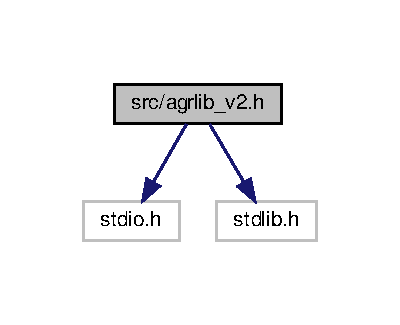
\includegraphics[width=192pt]{agrlib__v2_8h__incl}
\end{center}
\end{figure}
This graph shows which files directly or indirectly include this file\+:\nopagebreak
\begin{figure}[H]
\begin{center}
\leavevmode
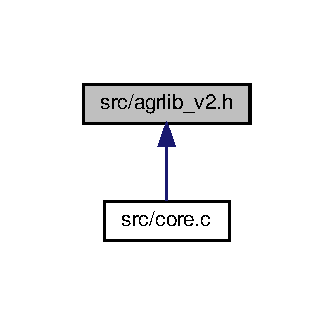
\includegraphics[width=160pt]{agrlib__v2_8h__dep__incl}
\end{center}
\end{figure}
\subsection*{Macros}
\begin{DoxyCompactItemize}
\item 
\#define \hyperlink{agrlib__v2_8h_a5ab5b9aaf3850b085ca39abf901b2751}{T\+E\+S\+T\+\_\+\+C\+A\+SE}
\begin{DoxyCompactList}\small\item\em For testing define T\+E\+S\+T\+\_\+\+C\+A\+SE. \end{DoxyCompactList}\item 
\#define \hyperlink{agrlib__v2_8h_abe6b865c045f3e7c6892ef4f15ff5779}{D\+O\+NE}~1
\begin{DoxyCompactList}\small\item\em D\+O\+NE is used as success indicator. \end{DoxyCompactList}\item 
\#define \hyperlink{agrlib__v2_8h_a8fe83ac76edc595f6b98cd4a4127aed5}{E\+R\+R\+OR}~0
\begin{DoxyCompactList}\small\item\em E\+R\+R\+OR is used as fail indicator. \end{DoxyCompactList}\end{DoxyCompactItemize}
\subsection*{Functions}
\begin{DoxyCompactItemize}
\item 
int \hyperlink{agrlib__v2_8h_a0307984afb426de0d910e5fc8eb5af27}{csv\+\_\+import} (char \hyperlink{core_8c_a4b2ae53d82dc2d82a6ba3d6488e3638f}{path\+\_\+to\+\_\+csv}\mbox{[}$\,$\mbox{]})
\begin{DoxyCompactList}\small\item\em Function perform import of file.\+Input value\+: path to file. Return value\+: D\+O\+NE or E\+R\+R\+OR. \end{DoxyCompactList}\item 
int \hyperlink{agrlib__v2_8h_a7a14e18fe42a95fdce291f1ffd1be5c2}{csv\+\_\+info} (char $\ast$\hyperlink{agrlib__v1_8h_ab00f83b047d06986d6709f8ac535b192}{csv})
\begin{DoxyCompactList}\small\item\em Function counts rows and columns, max length of line,also replace all E\+OL with N\+U\+LL. Input \+: pointer to csv in memory. Return value\+: D\+O\+NE or E\+R\+R\+OR. \end{DoxyCompactList}\item 
int \hyperlink{agrlib__v2_8h_a605396290960b729c55527ce1168deda}{init\+\_\+memory} (size\+\_\+t len, int case\+\_\+)
\item 
int \hyperlink{agrlib__v2_8h_aebc31f51013d2dc2c24e280b63e35c3f}{csv\+\_\+get\+\_\+lines} (char $\ast$\hyperlink{agrlib__v1_8h_ab00f83b047d06986d6709f8ac535b192}{csv})
\begin{DoxyCompactList}\small\item\em Function loops through file searching for line beginnings positions. Input \+: pointer to csv in memory. Return value\+: D\+O\+NE or E\+R\+R\+OR. \end{DoxyCompactList}\item 
int \hyperlink{agrlib__v2_8h_aadd713f59dccacdf303f1eae5ff3cbbe}{csv\+\_\+get\+\_\+timestamps} (char $\ast$\hyperlink{agrlib__v1_8h_ab00f83b047d06986d6709f8ac535b192}{csv})
\begin{DoxyCompactList}\small\item\em Function loops through file searching for timestamps positions. Input \+: pointer to csv in memory. Return value\+: D\+O\+NE or E\+R\+R\+OR. \end{DoxyCompactList}\item 
int \hyperlink{agrlib__v2_8h_a21172191aa50a1ec76d88e728f9c69d4}{sort\+\_\+timepointers} (char $\ast$$\ast$time, char $\ast$$\ast$line)
\begin{DoxyCompactList}\small\item\em Function sorts timestamps. Input \+: array of timestamps starts pointers and array of line beginnings. Algorithm\+: combo sorting. Return value\+: D\+O\+NE or E\+R\+R\+OR. \end{DoxyCompactList}\item 
int \hyperlink{agrlib__v2_8h_ab91f89f6a19d310763428e1bf599f4fe}{compare\+\_\+timestamps} (char $\ast$first, char $\ast$second)
\begin{DoxyCompactList}\small\item\em Function compares first given timespamp with second by subtraction. Return value\+: 1 for F$>$S., 2 for F$<$S., 3 for F=S or E\+R\+R\+OR. \end{DoxyCompactList}\item 
size\+\_\+t \hyperlink{agrlib__v2_8h_ad9931ba3f9b842cdf853e586e986ab50}{new\+\_\+gap} (size\+\_\+t gap)
\begin{DoxyCompactList}\small\item\em Function generates new gap for combo sort algorithm. Input \+: old gap. Return \+: new gap. \end{DoxyCompactList}\item 
char $\ast$$\ast$$\ast$ \hyperlink{agrlib__v2_8h_a5d809ffa3eb2e85f2e2a91b7feb39584}{agregate} (char $\ast$\hyperlink{core_8c_a4b2ae53d82dc2d82a6ba3d6488e3638f}{path\+\_\+to\+\_\+csv}, unsigned short int $\ast$timestamp\+\_\+column)
\begin{DoxyCompactList}\small\item\em Main function, controls order of program flow and. \end{DoxyCompactList}\item 
void \hyperlink{agrlib__v2_8h_a19ca95ef173bf8ed186fd3c4d0aede1f}{show\+\_\+hiden\+\_\+time} (char $\ast$timestamp)
\begin{DoxyCompactList}\small\item\em Help functions -\/ in test cases may come in handy. ! S\+T\+D\+O\+UT is used. \end{DoxyCompactList}\item 
void \hyperlink{agrlib__v2_8h_a4df9c8a3fc1c3470cdc57ecfb548fd95}{show\+\_\+hiden\+\_\+string} (char $\ast$line)
\begin{DoxyCompactList}\small\item\em Function prints line given by pointer until E\+OL met. \end{DoxyCompactList}\item 
void \hyperlink{agrlib__v2_8h_a93d82a5a51eb0de86f629e86dce96202}{general\+\_\+check} (int case\+\_\+)
\begin{DoxyCompactList}\small\item\em Function perform general check by printing\+: case\{1) -\/ all sorted timestamps, case(2) -\/ all sorted csv lines. \end{DoxyCompactList}\item 
int \hyperlink{agrlib__v2_8h_a8fd952fbab14a2eaaa9aaf96010e2aa0}{csv\+\_\+import} (char $\ast$\hyperlink{core_8c_a4b2ae53d82dc2d82a6ba3d6488e3638f}{path\+\_\+to\+\_\+csv})
\end{DoxyCompactItemize}
\subsection*{Variables}
\begin{DoxyCompactItemize}
\item 
char \hyperlink{agrlib__v2_8h_a2f44b091be60ccdd664997eb163d2ff4}{sep} = \textquotesingle{},\textquotesingle{}
\begin{DoxyCompactList}\small\item\em Defines csv separator, must be single symbol. \end{DoxyCompactList}\item 
int \hyperlink{agrlib__v2_8h_a4409b51f47ad8c26d98b227bf26bfbd9}{end\+\_\+\+CR} = 0x0D
\item 
int \hyperlink{agrlib__v2_8h_abb7d175ad428e618e66b9d002a475cf2}{end\+\_\+\+LF} = 0x0A
\begin{DoxyCompactList}\small\item\em End of line LF symbol. \end{DoxyCompactList}\item 
size\+\_\+t \hyperlink{agrlib__v2_8h_adfdc908b893f72ef73c8850671ba538f}{timestamp\+\_\+col} = 0
\begin{DoxyCompactList}\small\item\em This parameter is user defined. It holds the timestamps column number. Note, that columns are counted from 0 \+: 0,1,2,3,4, ... ,timestamp\+\_\+col, .... n. \end{DoxyCompactList}\item 
int \hyperlink{agrlib__v2_8h_aeed51c87c57a3eb984514da8000aeb7b}{timestamp\+\_\+len}
\item 
int \hyperlink{agrlib__v2_8h_a8466c885b251cd7cfa286745837b5347}{max\+\_\+try} = 5
\begin{DoxyCompactList}\small\item\em Max number of attempts to allocate memory. \end{DoxyCompactList}\item 
F\+I\+LE $\ast$ \hyperlink{agrlib__v2_8h_a82500a31718a0b612f28d06d2a448e04}{input\+\_\+csv}
\begin{DoxyCompactList}\small\item\em File pointer. \end{DoxyCompactList}\end{DoxyCompactItemize}


\subsection{Macro Definition Documentation}
\mbox{\Hypertarget{agrlib__v2_8h_abe6b865c045f3e7c6892ef4f15ff5779}\label{agrlib__v2_8h_abe6b865c045f3e7c6892ef4f15ff5779}} 
\index{agrlib\+\_\+v2.\+h@{agrlib\+\_\+v2.\+h}!D\+O\+NE@{D\+O\+NE}}
\index{D\+O\+NE@{D\+O\+NE}!agrlib\+\_\+v2.\+h@{agrlib\+\_\+v2.\+h}}
\subsubsection{\texorpdfstring{D\+O\+NE}{DONE}}
{\footnotesize\ttfamily \#define D\+O\+NE~1}



D\+O\+NE is used as success indicator. 

\mbox{\Hypertarget{agrlib__v2_8h_a8fe83ac76edc595f6b98cd4a4127aed5}\label{agrlib__v2_8h_a8fe83ac76edc595f6b98cd4a4127aed5}} 
\index{agrlib\+\_\+v2.\+h@{agrlib\+\_\+v2.\+h}!E\+R\+R\+OR@{E\+R\+R\+OR}}
\index{E\+R\+R\+OR@{E\+R\+R\+OR}!agrlib\+\_\+v2.\+h@{agrlib\+\_\+v2.\+h}}
\subsubsection{\texorpdfstring{E\+R\+R\+OR}{ERROR}}
{\footnotesize\ttfamily \#define E\+R\+R\+OR~0}



E\+R\+R\+OR is used as fail indicator. 

\mbox{\Hypertarget{agrlib__v2_8h_a5ab5b9aaf3850b085ca39abf901b2751}\label{agrlib__v2_8h_a5ab5b9aaf3850b085ca39abf901b2751}} 
\index{agrlib\+\_\+v2.\+h@{agrlib\+\_\+v2.\+h}!T\+E\+S\+T\+\_\+\+C\+A\+SE@{T\+E\+S\+T\+\_\+\+C\+A\+SE}}
\index{T\+E\+S\+T\+\_\+\+C\+A\+SE@{T\+E\+S\+T\+\_\+\+C\+A\+SE}!agrlib\+\_\+v2.\+h@{agrlib\+\_\+v2.\+h}}
\subsubsection{\texorpdfstring{T\+E\+S\+T\+\_\+\+C\+A\+SE}{TEST\_CASE}}
{\footnotesize\ttfamily \#define T\+E\+S\+T\+\_\+\+C\+A\+SE}



For testing define T\+E\+S\+T\+\_\+\+C\+A\+SE. 



\subsection{Function Documentation}
\mbox{\Hypertarget{agrlib__v2_8h_a5d809ffa3eb2e85f2e2a91b7feb39584}\label{agrlib__v2_8h_a5d809ffa3eb2e85f2e2a91b7feb39584}} 
\index{agrlib\+\_\+v2.\+h@{agrlib\+\_\+v2.\+h}!agregate@{agregate}}
\index{agregate@{agregate}!agrlib\+\_\+v2.\+h@{agrlib\+\_\+v2.\+h}}
\subsubsection{\texorpdfstring{agregate()}{agregate()}}
{\footnotesize\ttfamily char $\ast$$\ast$$\ast$ agregate (\begin{DoxyParamCaption}\item[{char $\ast$}]{path\+\_\+to\+\_\+csv,  }\item[{unsigned short int $\ast$}]{timestamp\+\_\+column }\end{DoxyParamCaption})}



Main function, controls order of program flow and. 

This is main logic function. Call this with path to perform all. Program flow \+: csv\+\_\+import ---$>$ csv\+\_\+info --$>$ init\+\_\+memory ---$>$ csv\+\_\+get\+\_\+lines ---$>$ csv\+\_\+get\+\_\+timestamps ---$>$ sort(compare) E\+ND file import ---$>$ general information --$>$ memory initialization ---$>$ lines search ---$>$ timestamps search ---$>$ sorting E\+ND Information about timestamp column is taken from user. \mbox{\Hypertarget{agrlib__v2_8h_ab91f89f6a19d310763428e1bf599f4fe}\label{agrlib__v2_8h_ab91f89f6a19d310763428e1bf599f4fe}} 
\index{agrlib\+\_\+v2.\+h@{agrlib\+\_\+v2.\+h}!compare\+\_\+timestamps@{compare\+\_\+timestamps}}
\index{compare\+\_\+timestamps@{compare\+\_\+timestamps}!agrlib\+\_\+v2.\+h@{agrlib\+\_\+v2.\+h}}
\subsubsection{\texorpdfstring{compare\+\_\+timestamps()}{compare\_timestamps()}}
{\footnotesize\ttfamily int compare\+\_\+timestamps (\begin{DoxyParamCaption}\item[{char $\ast$}]{first,  }\item[{char $\ast$}]{second }\end{DoxyParamCaption})}



Function compares first given timespamp with second by subtraction. Return value\+: 1 for F$>$S., 2 for F$<$S., 3 for F=S or E\+R\+R\+OR. 

Comparison is done by subtraction and comparison with zero, so it is important to follow timestamps format Return value 1 if first(passed value) $>$ second (passed value) 2 if first $<$ second 3 if first = second In T\+E\+S\+T\+\_\+\+C\+A\+SE some additional information is shown

Comparing we loop through timestamps subtracting values Return values reflects relations between First and Second values \mbox{\Hypertarget{agrlib__v2_8h_aebc31f51013d2dc2c24e280b63e35c3f}\label{agrlib__v2_8h_aebc31f51013d2dc2c24e280b63e35c3f}} 
\index{agrlib\+\_\+v2.\+h@{agrlib\+\_\+v2.\+h}!csv\+\_\+get\+\_\+lines@{csv\+\_\+get\+\_\+lines}}
\index{csv\+\_\+get\+\_\+lines@{csv\+\_\+get\+\_\+lines}!agrlib\+\_\+v2.\+h@{agrlib\+\_\+v2.\+h}}
\subsubsection{\texorpdfstring{csv\+\_\+get\+\_\+lines()}{csv\_get\_lines()}}
{\footnotesize\ttfamily int csv\+\_\+get\+\_\+lines (\begin{DoxyParamCaption}\item[{char $\ast$}]{csv }\end{DoxyParamCaption})}



Function loops through file searching for line beginnings positions. Input \+: pointer to csv in memory. Return value\+: D\+O\+NE or E\+R\+R\+OR. 

Getting lines beginnings starts with memory allocation. We need memory for pointers array with length equal to the number of rows

In case of fail we will try up try max try number

Then we search for position of each first not null symbol and save reference on it \mbox{\Hypertarget{agrlib__v2_8h_aadd713f59dccacdf303f1eae5ff3cbbe}\label{agrlib__v2_8h_aadd713f59dccacdf303f1eae5ff3cbbe}} 
\index{agrlib\+\_\+v2.\+h@{agrlib\+\_\+v2.\+h}!csv\+\_\+get\+\_\+timestamps@{csv\+\_\+get\+\_\+timestamps}}
\index{csv\+\_\+get\+\_\+timestamps@{csv\+\_\+get\+\_\+timestamps}!agrlib\+\_\+v2.\+h@{agrlib\+\_\+v2.\+h}}
\subsubsection{\texorpdfstring{csv\+\_\+get\+\_\+timestamps()}{csv\_get\_timestamps()}}
{\footnotesize\ttfamily int csv\+\_\+get\+\_\+timestamps (\begin{DoxyParamCaption}\item[{char $\ast$}]{csv }\end{DoxyParamCaption})}



Function loops through file searching for timestamps positions. Input \+: pointer to csv in memory. Return value\+: D\+O\+NE or E\+R\+R\+OR. 

Getting timestamps pointers for further comparison start with memory a allocation. We try to allocate memory as well several times

To indicate if current position in file contains timestamp or not we will count columns If file contains an error and we exceed the number of columns -\/work stops.

As timestamp is found and its first character address is stored -\/ we do not expect timestamps in this line any more

All timestamps should be the same length, which is never exceeded during timestamps comparison

Header does not take part in counting, so first -\/ we must pass it

To avoid errors in column number we indicate step from meaningful part to meaning less If at this moments we did not met enough separators -\/ error

Each symbol is checked for separator or E\+OL

E\+OL means that we are in useless part

If timestamp is located at the end of line -\/ its length is counted here.

As well at the end of line we check for number of columns to be the same as counted in header

Another error is reaching end of line and without reaching timestamp column.

Indication of non header line is \+: timestamp length counting has started, but header\+\_\+passed is still false .

Next error is different length of timestamps, which means that error if no timestamp found. If something else is in column of ts, but of the same length -\/ it ok, as well it will be sorted.

Length of timestamp is as well controlled/counted when separator is met.

Finally -\/ an address of first symbol in timestamps columns is taken. \mbox{\Hypertarget{agrlib__v2_8h_a0307984afb426de0d910e5fc8eb5af27}\label{agrlib__v2_8h_a0307984afb426de0d910e5fc8eb5af27}} 
\index{agrlib\+\_\+v2.\+h@{agrlib\+\_\+v2.\+h}!csv\+\_\+import@{csv\+\_\+import}}
\index{csv\+\_\+import@{csv\+\_\+import}!agrlib\+\_\+v2.\+h@{agrlib\+\_\+v2.\+h}}
\subsubsection{\texorpdfstring{csv\+\_\+import()}{csv\_import()}\hspace{0.1cm}{\footnotesize\ttfamily [1/2]}}
{\footnotesize\ttfamily int csv\+\_\+import (\begin{DoxyParamCaption}\item[{char}]{path\+\_\+to\+\_\+csv\mbox{[}$\,$\mbox{]} }\end{DoxyParamCaption})}



Function perform import of file.\+Input value\+: path to file. Return value\+: D\+O\+NE or E\+R\+R\+OR. 

\mbox{\Hypertarget{agrlib__v2_8h_a8fd952fbab14a2eaaa9aaf96010e2aa0}\label{agrlib__v2_8h_a8fd952fbab14a2eaaa9aaf96010e2aa0}} 
\index{agrlib\+\_\+v2.\+h@{agrlib\+\_\+v2.\+h}!csv\+\_\+import@{csv\+\_\+import}}
\index{csv\+\_\+import@{csv\+\_\+import}!agrlib\+\_\+v2.\+h@{agrlib\+\_\+v2.\+h}}
\subsubsection{\texorpdfstring{csv\+\_\+import()}{csv\_import()}\hspace{0.1cm}{\footnotesize\ttfamily [2/2]}}
{\footnotesize\ttfamily int csv\+\_\+import (\begin{DoxyParamCaption}\item[{char $\ast$}]{path\+\_\+to\+\_\+csv }\end{DoxyParamCaption})}

Import starts with reading file. An E\+R\+R\+OR returned in case of fail.

The first thing after file was opened -\/ get its size. Then we allocate memory. All at once.

To free memory lets save the original reference

If we have memory -\/ read whole file to it and then close file

If at some stage an error occurs -\/ E\+R\+R\+OR is returned end the program generaly ends. Possible errors\+: read less than file size(import error), not enough memory to hold file(mem error), error in opening file. These are end cases and E\+R\+R\+OR is returned. However we will consider an empty file as already sorted and return D\+O\+NE\mbox{\Hypertarget{agrlib__v2_8h_a7a14e18fe42a95fdce291f1ffd1be5c2}\label{agrlib__v2_8h_a7a14e18fe42a95fdce291f1ffd1be5c2}} 
\index{agrlib\+\_\+v2.\+h@{agrlib\+\_\+v2.\+h}!csv\+\_\+info@{csv\+\_\+info}}
\index{csv\+\_\+info@{csv\+\_\+info}!agrlib\+\_\+v2.\+h@{agrlib\+\_\+v2.\+h}}
\subsubsection{\texorpdfstring{csv\+\_\+info()}{csv\_info()}}
{\footnotesize\ttfamily int csv\+\_\+info (\begin{DoxyParamCaption}\item[{char $\ast$}]{csv }\end{DoxyParamCaption})}



Function counts rows and columns, max length of line,also replace all E\+OL with N\+U\+LL. Input \+: pointer to csv in memory. Return value\+: D\+O\+NE or E\+R\+R\+OR. 

First,lets count columns. For this we use first line, as it is considered to be header

So, each character is compared with separator or E\+OL

Each found separator increase column number

As the E\+OL reached -\/ we increase column number again \+: ... , ... , ... has 3 col, but only 2 separators

Here we will also check if file contains more than one line.

If only one line found -\/ we return, as it has no reason to continue sorting

Next -\/ count meaningful lines and maximum line length. From here line becomes sequence of characters delimited by \textquotesingle{}\textbackslash{}0\textquotesingle{} (max\+\_\+len -\/ maximum length, cur\+\_\+len -\/ current length)

Replacing all E\+OL with \textquotesingle{}\textbackslash{}0\textquotesingle{} will make searching easier

In test case, information about file will be printed \mbox{\Hypertarget{agrlib__v2_8h_a93d82a5a51eb0de86f629e86dce96202}\label{agrlib__v2_8h_a93d82a5a51eb0de86f629e86dce96202}} 
\index{agrlib\+\_\+v2.\+h@{agrlib\+\_\+v2.\+h}!general\+\_\+check@{general\+\_\+check}}
\index{general\+\_\+check@{general\+\_\+check}!agrlib\+\_\+v2.\+h@{agrlib\+\_\+v2.\+h}}
\subsubsection{\texorpdfstring{general\+\_\+check()}{general\_check()}}
{\footnotesize\ttfamily void general\+\_\+check (\begin{DoxyParamCaption}\item[{int}]{case\+\_\+ }\end{DoxyParamCaption})}



Function perform general check by printing\+: case\{1) -\/ all sorted timestamps, case(2) -\/ all sorted csv lines. 

Shows all timestamps(1), saved by pointers or lines(2), saved by pointers \mbox{\Hypertarget{agrlib__v2_8h_a605396290960b729c55527ce1168deda}\label{agrlib__v2_8h_a605396290960b729c55527ce1168deda}} 
\index{agrlib\+\_\+v2.\+h@{agrlib\+\_\+v2.\+h}!init\+\_\+memory@{init\+\_\+memory}}
\index{init\+\_\+memory@{init\+\_\+memory}!agrlib\+\_\+v2.\+h@{agrlib\+\_\+v2.\+h}}
\subsubsection{\texorpdfstring{init\+\_\+memory()}{init\_memory()}}
{\footnotesize\ttfamily int init\+\_\+memory (\begin{DoxyParamCaption}\item[{size\+\_\+t}]{len,  }\item[{int}]{case\+\_\+ }\end{DoxyParamCaption})}

Function contains main memory initialization. Input\+: size to initialize pointer with(main case -\/ number of rows) and cases 1-\/2-\/3, which pointer to initialize with memory. Return value\+: D\+O\+NE or E\+R\+R\+OR For better structure some memory initialization is located here. Global pointers timestamp and lines getting memory from here. Input\+: len -\/ size of memory to allocate, case\+\_\+ -\/ for which pointer(1,2,3) \mbox{\Hypertarget{agrlib__v2_8h_ad9931ba3f9b842cdf853e586e986ab50}\label{agrlib__v2_8h_ad9931ba3f9b842cdf853e586e986ab50}} 
\index{agrlib\+\_\+v2.\+h@{agrlib\+\_\+v2.\+h}!new\+\_\+gap@{new\+\_\+gap}}
\index{new\+\_\+gap@{new\+\_\+gap}!agrlib\+\_\+v2.\+h@{agrlib\+\_\+v2.\+h}}
\subsubsection{\texorpdfstring{new\+\_\+gap()}{new\_gap()}}
{\footnotesize\ttfamily size\+\_\+t new\+\_\+gap (\begin{DoxyParamCaption}\item[{size\+\_\+t}]{gap }\end{DoxyParamCaption})}



Function generates new gap for combo sort algorithm. Input \+: old gap. Return \+: new gap. 

New gap for sorting is formed from rows number and after first loop of algorithm from last gap. Conditions of gap formation could be changed \mbox{\Hypertarget{agrlib__v2_8h_a4df9c8a3fc1c3470cdc57ecfb548fd95}\label{agrlib__v2_8h_a4df9c8a3fc1c3470cdc57ecfb548fd95}} 
\index{agrlib\+\_\+v2.\+h@{agrlib\+\_\+v2.\+h}!show\+\_\+hiden\+\_\+string@{show\+\_\+hiden\+\_\+string}}
\index{show\+\_\+hiden\+\_\+string@{show\+\_\+hiden\+\_\+string}!agrlib\+\_\+v2.\+h@{agrlib\+\_\+v2.\+h}}
\subsubsection{\texorpdfstring{show\+\_\+hiden\+\_\+string()}{show\_hiden\_string()}}
{\footnotesize\ttfamily void show\+\_\+hiden\+\_\+string (\begin{DoxyParamCaption}\item[{char $\ast$}]{line }\end{DoxyParamCaption})}



Function prints line given by pointer until E\+OL met. 

Helpful when testing. Show line by its pointer \mbox{\Hypertarget{agrlib__v2_8h_a19ca95ef173bf8ed186fd3c4d0aede1f}\label{agrlib__v2_8h_a19ca95ef173bf8ed186fd3c4d0aede1f}} 
\index{agrlib\+\_\+v2.\+h@{agrlib\+\_\+v2.\+h}!show\+\_\+hiden\+\_\+time@{show\+\_\+hiden\+\_\+time}}
\index{show\+\_\+hiden\+\_\+time@{show\+\_\+hiden\+\_\+time}!agrlib\+\_\+v2.\+h@{agrlib\+\_\+v2.\+h}}
\subsubsection{\texorpdfstring{show\+\_\+hiden\+\_\+time()}{show\_hiden\_time()}}
{\footnotesize\ttfamily void show\+\_\+hiden\+\_\+time (\begin{DoxyParamCaption}\item[{char $\ast$}]{timestamp }\end{DoxyParamCaption})}



Help functions -\/ in test cases may come in handy. ! S\+T\+D\+O\+UT is used. 

Function prints timestamp, given by pointer, of length timestamp\+\_\+len Helpful when testing. Show timestamps by pointer \mbox{\Hypertarget{agrlib__v2_8h_a21172191aa50a1ec76d88e728f9c69d4}\label{agrlib__v2_8h_a21172191aa50a1ec76d88e728f9c69d4}} 
\index{agrlib\+\_\+v2.\+h@{agrlib\+\_\+v2.\+h}!sort\+\_\+timepointers@{sort\+\_\+timepointers}}
\index{sort\+\_\+timepointers@{sort\+\_\+timepointers}!agrlib\+\_\+v2.\+h@{agrlib\+\_\+v2.\+h}}
\subsubsection{\texorpdfstring{sort\+\_\+timepointers()}{sort\_timepointers()}}
{\footnotesize\ttfamily int sort\+\_\+timepointers (\begin{DoxyParamCaption}\item[{char $\ast$$\ast$}]{time,  }\item[{char $\ast$$\ast$}]{line }\end{DoxyParamCaption})}



Function sorts timestamps. Input \+: array of timestamps starts pointers and array of line beginnings. Algorithm\+: combo sorting. Return value\+: D\+O\+NE or E\+R\+R\+OR. 

Algorithm is based on bubble sort. The only difference is in shrinking gap between two compared values. At last stages it becomes pure bubble sort.

Before comparison we would check if it worth to be done -\/ if csv has only 2 rows it has no meaning.

In other case, first thing to do -\/ step over header.

Then define some temporary holders for compared objects We compare timestamps but the line order gets changed too

Sorting loop starts with getting new gap

Then we compare two timestamps with compare\+\_\+timestamps function. IF Y\+OU N\+E\+ED TO C\+H\+A\+N\+GE O\+R\+D\+ER -\/ S\+ET 2 I\+N\+S\+T\+E\+AD OF 1 IN IF C\+O\+N\+D\+I\+T\+I\+ON If the order is ok, go on, else -\/ swap the pointers 

\subsection{Variable Documentation}
\mbox{\Hypertarget{agrlib__v2_8h_a4409b51f47ad8c26d98b227bf26bfbd9}\label{agrlib__v2_8h_a4409b51f47ad8c26d98b227bf26bfbd9}} 
\index{agrlib\+\_\+v2.\+h@{agrlib\+\_\+v2.\+h}!end\+\_\+\+CR@{end\+\_\+\+CR}}
\index{end\+\_\+\+CR@{end\+\_\+\+CR}!agrlib\+\_\+v2.\+h@{agrlib\+\_\+v2.\+h}}
\subsubsection{\texorpdfstring{end\+\_\+\+CR}{end\_CR}}
{\footnotesize\ttfamily int end\+\_\+\+CR = 0x0D}

To handle different OS dependent E\+OL, E\+OL symbols defined End of line CR symbol \mbox{\Hypertarget{agrlib__v2_8h_abb7d175ad428e618e66b9d002a475cf2}\label{agrlib__v2_8h_abb7d175ad428e618e66b9d002a475cf2}} 
\index{agrlib\+\_\+v2.\+h@{agrlib\+\_\+v2.\+h}!end\+\_\+\+LF@{end\+\_\+\+LF}}
\index{end\+\_\+\+LF@{end\+\_\+\+LF}!agrlib\+\_\+v2.\+h@{agrlib\+\_\+v2.\+h}}
\subsubsection{\texorpdfstring{end\+\_\+\+LF}{end\_LF}}
{\footnotesize\ttfamily int end\+\_\+\+LF = 0x0A}



End of line LF symbol. 

\mbox{\Hypertarget{agrlib__v2_8h_a82500a31718a0b612f28d06d2a448e04}\label{agrlib__v2_8h_a82500a31718a0b612f28d06d2a448e04}} 
\index{agrlib\+\_\+v2.\+h@{agrlib\+\_\+v2.\+h}!input\+\_\+csv@{input\+\_\+csv}}
\index{input\+\_\+csv@{input\+\_\+csv}!agrlib\+\_\+v2.\+h@{agrlib\+\_\+v2.\+h}}
\subsubsection{\texorpdfstring{input\+\_\+csv}{input\_csv}}
{\footnotesize\ttfamily F\+I\+LE$\ast$ input\+\_\+csv}



File pointer. 

\mbox{\Hypertarget{agrlib__v2_8h_a8466c885b251cd7cfa286745837b5347}\label{agrlib__v2_8h_a8466c885b251cd7cfa286745837b5347}} 
\index{agrlib\+\_\+v2.\+h@{agrlib\+\_\+v2.\+h}!max\+\_\+try@{max\+\_\+try}}
\index{max\+\_\+try@{max\+\_\+try}!agrlib\+\_\+v2.\+h@{agrlib\+\_\+v2.\+h}}
\subsubsection{\texorpdfstring{max\+\_\+try}{max\_try}}
{\footnotesize\ttfamily int max\+\_\+try = 5}



Max number of attempts to allocate memory. 

\mbox{\Hypertarget{agrlib__v2_8h_a2f44b091be60ccdd664997eb163d2ff4}\label{agrlib__v2_8h_a2f44b091be60ccdd664997eb163d2ff4}} 
\index{agrlib\+\_\+v2.\+h@{agrlib\+\_\+v2.\+h}!sep@{sep}}
\index{sep@{sep}!agrlib\+\_\+v2.\+h@{agrlib\+\_\+v2.\+h}}
\subsubsection{\texorpdfstring{sep}{sep}}
{\footnotesize\ttfamily char sep = \textquotesingle{},\textquotesingle{}}



Defines csv separator, must be single symbol. 

General \+: first meaningfull line is header for table Empty lines are allowed \mbox{\Hypertarget{agrlib__v2_8h_adfdc908b893f72ef73c8850671ba538f}\label{agrlib__v2_8h_adfdc908b893f72ef73c8850671ba538f}} 
\index{agrlib\+\_\+v2.\+h@{agrlib\+\_\+v2.\+h}!timestamp\+\_\+col@{timestamp\+\_\+col}}
\index{timestamp\+\_\+col@{timestamp\+\_\+col}!agrlib\+\_\+v2.\+h@{agrlib\+\_\+v2.\+h}}
\subsubsection{\texorpdfstring{timestamp\+\_\+col}{timestamp\_col}}
{\footnotesize\ttfamily size\+\_\+t timestamp\+\_\+col = 0}



This parameter is user defined. It holds the timestamps column number. Note, that columns are counted from 0 \+: 0,1,2,3,4, ... ,timestamp\+\_\+col, .... n. 

\mbox{\Hypertarget{agrlib__v2_8h_aeed51c87c57a3eb984514da8000aeb7b}\label{agrlib__v2_8h_aeed51c87c57a3eb984514da8000aeb7b}} 
\index{agrlib\+\_\+v2.\+h@{agrlib\+\_\+v2.\+h}!timestamp\+\_\+len@{timestamp\+\_\+len}}
\index{timestamp\+\_\+len@{timestamp\+\_\+len}!agrlib\+\_\+v2.\+h@{agrlib\+\_\+v2.\+h}}
\subsubsection{\texorpdfstring{timestamp\+\_\+len}{timestamp\_len}}
{\footnotesize\ttfamily int timestamp\+\_\+len}

Program accepts all ,constant length, timestamps which are following the I\+SO 8601 (\href{https://en.wikipedia.org/wiki/ISO_8601}{\tt https\+://en.\+wikipedia.\+org/wiki/\+I\+S\+O\+\_\+8601}). Length is counted automatically (all symb. included) 
\hypertarget{core_8c}{}\section{src/core.c File Reference}
\label{core_8c}\index{src/core.\+c@{src/core.\+c}}
{\ttfamily \#include $<$kore/kore.\+h$>$}\newline
{\ttfamily \#include $<$kore/http.\+h$>$}\newline
{\ttfamily \#include $<$kore/pgsql.\+h$>$}\newline
{\ttfamily \#include $<$libintl.\+h$>$}\newline
{\ttfamily \#include $<$locale.\+h$>$}\newline
{\ttfamily \#include \char`\"{}agrlib\+\_\+v2.\+h\char`\"{}}\newline
Include dependency graph for core.\+c\+:\nopagebreak
\begin{figure}[H]
\begin{center}
\leavevmode
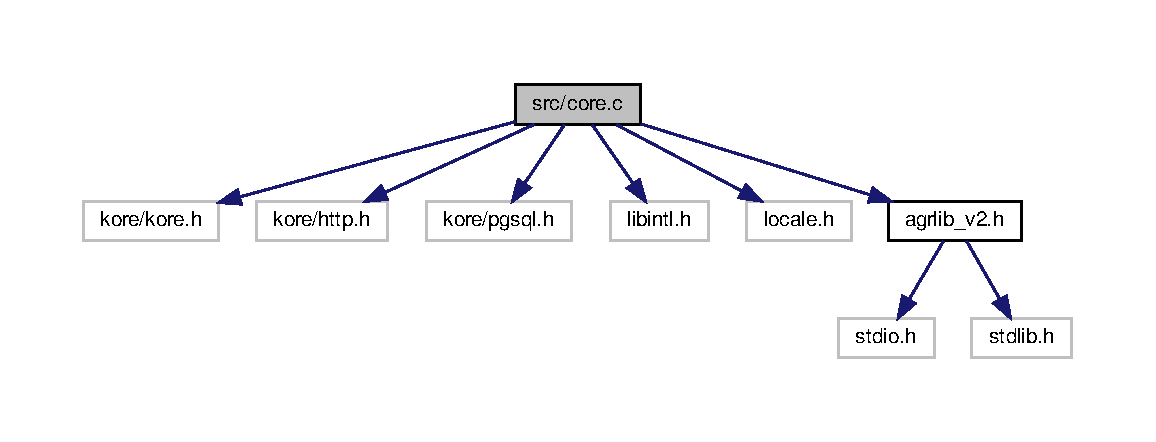
\includegraphics[width=350pt]{core_8c__incl}
\end{center}
\end{figure}
\subsection*{Macros}
\begin{DoxyCompactItemize}
\item 
\#define \hyperlink{core_8c_ab92bb4161a6308b302d283816975c3a6}{\+\_\+}(S\+T\+R\+I\+NG)~gettext(S\+T\+R\+I\+NG)
\item 
\#define \hyperlink{core_8c_a5ab5b9aaf3850b085ca39abf901b2751}{T\+E\+S\+T\+\_\+\+C\+A\+SE}
\begin{DoxyCompactList}\small\item\em Define T\+E\+S\+T\+\_\+\+C\+A\+SE to perfom output to stdout when debuging or testing. \end{DoxyCompactList}\item 
\#define \hyperlink{core_8c_a22e00999d254cceeb29d2a858b432e41}{\+\_\+}(A)~gettext(A)
\item 
\#define \hyperlink{core_8c_a8db4f72cfa2b36aba553c8fd1ab6af9e}{L\+O\+C\+A\+L\+E\+\_\+\+D\+IR}~\char`\"{}locale\char`\"{}
\begin{DoxyCompactList}\small\item\em For l18n -\/ define here the directory with .mo files. \end{DoxyCompactList}\item 
\#define \hyperlink{core_8c_aca8570fb706c81df371b7f9bc454ae03}{P\+A\+C\+K\+A\+GE}~\char`\"{}core\char`\"{}
\begin{DoxyCompactList}\small\item\em Define here the name of file.\+mo to use. \end{DoxyCompactList}\end{DoxyCompactItemize}
\subsection*{Functions}
\begin{DoxyCompactItemize}
\item 
int \hyperlink{core_8c_a63c2c93fc1421e2956860a788fce8617}{init} (int state)
\begin{DoxyCompactList}\small\item\em Register database. \end{DoxyCompactList}\item 
int \hyperlink{core_8c_a6543687223c9eafbac413e52ddd2da7b}{page} (struct http\+\_\+request $\ast$)
\begin{DoxyCompactList}\small\item\em Dealing with request. \end{DoxyCompactList}\item 
int \hyperlink{core_8c_a0939e2f18610176aada23a5961ce7ecd}{form\+\_\+response} (struct kore\+\_\+buf $\ast$buf, char $\ast$$\ast$table\+\_\+sorted)
\begin{DoxyCompactList}\small\item\em Forms html response, but does not send it. Table is formed from \textquotesingle{}table\+\_\+sorted\textquotesingle{}. \end{DoxyCompactList}\item 
int \hyperlink{core_8c_af8192996f3c522f10ab475ec2b6e6f4a}{form\+\_\+and\+\_\+fire\+\_\+query} (struct kore\+\_\+buf $\ast$qr\+\_\+buf, struct kore\+\_\+pgsql $\ast$sql, char $\ast$line)
\begin{DoxyCompactList}\small\item\em Responsible for quering database with I\+N\+S\+E\+RT commands. \end{DoxyCompactList}\item 
int \hyperlink{core_8c_a9f53c2262b7acaa2b5a1e1d2463f14f1}{setup\+\_\+conn} (struct kore\+\_\+pgsql $\ast$sql)
\begin{DoxyCompactList}\small\item\em Sets up / opens connection with database. \end{DoxyCompactList}\item 
int \hyperlink{core_8c_ab3444f46f7643490834531d552454bcd}{create\+\_\+table\+\_\+if\+\_\+notexist} (char $\ast$csv\+\_\+header, struct kore\+\_\+pgsql $\ast$sql)
\begin{DoxyCompactList}\small\item\em Creates table if not exist. \end{DoxyCompactList}\item 
int \hyperlink{core_8c_a50873f71312e18a4e1eeb8b30c4b755f}{database\+\_\+query} (struct kore\+\_\+pgsql $\ast$sql, char $\ast$$\ast$table\+\_\+sorted)
\begin{DoxyCompactList}\small\item\em Sets up database connection, performs all queries. \end{DoxyCompactList}\end{DoxyCompactItemize}
\subsection*{Variables}
\begin{DoxyCompactItemize}
\item 
char \hyperlink{core_8c_a519c8e500ba2ea066c723ee28e30fa04}{html\+\_\+table} \mbox{[}$\,$\mbox{]} = \char`\"{}$<$!D\+O\+C\+T\+Y\+PE html$>$$<$html$>$$<$head$>$$<$meta charset=\textbackslash{}\char`\"{}U\+TF-\/8\textbackslash{}\char`\"{}$>$$<$style$>$table\{font-\/family\+: arial, sans-\/serif;border-\/collapse\+: collapse;width\+: 100\%;\}td, th \{border\+: 1px solid \#dddddd;text-\/align\+: left;padding\+: 8px;\}tr\+:nth-\/child(even) \{background-\/color\+: \#dddddd;\}$<$/style$>$$<$/head$>$$<$body$>$$<$h2$>$\+R\+E\+S\+U\+L\+T\+S$<$/h2$>$$<$table$>$\char`\"{}
\begin{DoxyCompactList}\small\item\em Tamplate for generated H\+T\+ML table. \end{DoxyCompactList}\item 
char \hyperlink{core_8c_aba77d446d3c6b20fc708dbaa56669a8d}{error\+\_\+response\+\_\+header} \mbox{[}$\,$\mbox{]} = \char`\"{}$<$!D\+O\+C\+T\+Y\+PE html$>$$<$html$>$$<$head$>$$<$meta charset=\textbackslash{}\char`\"{}utf-\/8\textbackslash{}\char`\"{}$>$$<$/head$>$$<$body$>$L\+O\+G\+:\char`\"{}
\begin{DoxyCompactList}\small\item\em Tamplate for generated H\+T\+ML error response. \end{DoxyCompactList}\item 
char \hyperlink{core_8c_a56c55320a85231784cb14d45e6d8043a}{error\+\_\+response\+\_\+end} \mbox{[}$\,$\mbox{]} = \char`\"{}$<$/body$>$$<$/html$>$\char`\"{}
\item 
char \hyperlink{core_8c_a88018c0aba001bc30dd2bf70c5098c02}{html\+\_\+table\+\_\+end} \mbox{[}$\,$\mbox{]} = \char`\"{}$<$/table$>$$<$/body$>$$<$/html$>$\char`\"{}
\begin{DoxyCompactList}\small\item\em End of table. \end{DoxyCompactList}\item 
char \hyperlink{core_8c_a1bffe9444fb0c41cb785eef0ceb29a8d}{conn\+\_\+str} \mbox{[}$\,$\mbox{]} = \char`\"{}host=localhost dbname=your\+\_\+database\+\_\+name user=example\+\_\+user password=example\char`\"{}
\begin{DoxyCompactList}\small\item\em Main connection string, fill with your parametrs according to P\+G\+S\+QL connection string rules. \end{DoxyCompactList}\item 
char $\ast$ \hyperlink{core_8c_ab013af67ba953d509575c86d9e65da44}{table\+\_\+name}
\begin{DoxyCompactList}\small\item\em Table name to use if it is not created from file name(\+C\+R\+E\+A\+T\+E\+\_\+\+N\+A\+M\+E\+\_\+\+F\+R\+O\+M\+\_\+\+F\+I\+L\+E not defined) \end{DoxyCompactList}\item 
char \hyperlink{core_8c_ac6415df1e2eb068fae92d9ec1dab1702}{max\+\_\+entry\+\_\+size} \mbox{[}$\,$\mbox{]} = \char`\"{} varchar(40) \char`\"{}
\begin{DoxyCompactList}\small\item\em If table is new created, each entry is treated as text(varchar). Here is max size of each entry. \end{DoxyCompactList}\item 
char \hyperlink{core_8c_a706bc0a919ca845fc1f5c8f58074e924}{ts\+\_\+in\+\_\+db} \mbox{[}$\,$\mbox{]} = \char`\"{} timestamp \char`\"{}
\begin{DoxyCompactList}\small\item\em This key is used for column with timestamp, if database is created. \end{DoxyCompactList}\item 
char $\ast$ \hyperlink{core_8c_a4b2ae53d82dc2d82a6ba3d6488e3638f}{path\+\_\+to\+\_\+csv}
\item 
int \hyperlink{core_8c_abc370adb7e2af08ae0ab13964d45d1c4}{max\+\_\+try\+\_\+conn} = 5
\begin{DoxyCompactList}\small\item\em Holds the number of attempts to do, when trying to access database. \end{DoxyCompactList}\item 
int \hyperlink{core_8c_a6b9a9c1be87e8344b94882f91f56805b}{escape\+\_\+needed} = 1
\begin{DoxyCompactList}\small\item\em This flag wraps query in \$\$ for escaping some characters(like quots) \end{DoxyCompactList}\item 
int \hyperlink{core_8c_ad25499646dfc76b1dfafbe258ea21f19}{form\+\_\+name\+\_\+from\+\_\+path} = 1
\begin{DoxyCompactList}\small\item\em If no name was suplied to create table with and this flag is up -\/ we will get name from file. \end{DoxyCompactList}\item 
int \hyperlink{core_8c_a299efd1f0f06729d349e9c000260a4a1}{name\+\_\+len} = 0
\end{DoxyCompactItemize}


\subsection{Macro Definition Documentation}
\mbox{\Hypertarget{core_8c_ab92bb4161a6308b302d283816975c3a6}\label{core_8c_ab92bb4161a6308b302d283816975c3a6}} 
\index{core.\+c@{core.\+c}!\+\_\+@{\+\_\+}}
\index{\+\_\+@{\+\_\+}!core.\+c@{core.\+c}}
\subsubsection{\texorpdfstring{\+\_\+}{\_}\hspace{0.1cm}{\footnotesize\ttfamily [1/2]}}
{\footnotesize\ttfamily \#define \+\_\+(\begin{DoxyParamCaption}\item[{}]{S\+T\+R\+I\+NG }\end{DoxyParamCaption})~gettext(S\+T\+R\+I\+NG)}

\begin{DoxyAuthor}{Author}
Cherniaev Egor 
\end{DoxyAuthor}
\mbox{\Hypertarget{core_8c_a22e00999d254cceeb29d2a858b432e41}\label{core_8c_a22e00999d254cceeb29d2a858b432e41}} 
\index{core.\+c@{core.\+c}!\+\_\+@{\+\_\+}}
\index{\+\_\+@{\+\_\+}!core.\+c@{core.\+c}}
\subsubsection{\texorpdfstring{\+\_\+}{\_}\hspace{0.1cm}{\footnotesize\ttfamily [2/2]}}
{\footnotesize\ttfamily \#define \+\_\+(\begin{DoxyParamCaption}\item[{}]{A }\end{DoxyParamCaption})~gettext(A)}

\begin{DoxyAuthor}{Author}
Cherniaev Egor 
\end{DoxyAuthor}
\mbox{\Hypertarget{core_8c_a8db4f72cfa2b36aba553c8fd1ab6af9e}\label{core_8c_a8db4f72cfa2b36aba553c8fd1ab6af9e}} 
\index{core.\+c@{core.\+c}!L\+O\+C\+A\+L\+E\+\_\+\+D\+IR@{L\+O\+C\+A\+L\+E\+\_\+\+D\+IR}}
\index{L\+O\+C\+A\+L\+E\+\_\+\+D\+IR@{L\+O\+C\+A\+L\+E\+\_\+\+D\+IR}!core.\+c@{core.\+c}}
\subsubsection{\texorpdfstring{L\+O\+C\+A\+L\+E\+\_\+\+D\+IR}{LOCALE\_DIR}}
{\footnotesize\ttfamily \#define L\+O\+C\+A\+L\+E\+\_\+\+D\+IR~\char`\"{}locale\char`\"{}}



For l18n -\/ define here the directory with .mo files. 

\mbox{\Hypertarget{core_8c_aca8570fb706c81df371b7f9bc454ae03}\label{core_8c_aca8570fb706c81df371b7f9bc454ae03}} 
\index{core.\+c@{core.\+c}!P\+A\+C\+K\+A\+GE@{P\+A\+C\+K\+A\+GE}}
\index{P\+A\+C\+K\+A\+GE@{P\+A\+C\+K\+A\+GE}!core.\+c@{core.\+c}}
\subsubsection{\texorpdfstring{P\+A\+C\+K\+A\+GE}{PACKAGE}}
{\footnotesize\ttfamily \#define P\+A\+C\+K\+A\+GE~\char`\"{}core\char`\"{}}



Define here the name of file.\+mo to use. 

\mbox{\Hypertarget{core_8c_a5ab5b9aaf3850b085ca39abf901b2751}\label{core_8c_a5ab5b9aaf3850b085ca39abf901b2751}} 
\index{core.\+c@{core.\+c}!T\+E\+S\+T\+\_\+\+C\+A\+SE@{T\+E\+S\+T\+\_\+\+C\+A\+SE}}
\index{T\+E\+S\+T\+\_\+\+C\+A\+SE@{T\+E\+S\+T\+\_\+\+C\+A\+SE}!core.\+c@{core.\+c}}
\subsubsection{\texorpdfstring{T\+E\+S\+T\+\_\+\+C\+A\+SE}{TEST\_CASE}}
{\footnotesize\ttfamily \#define T\+E\+S\+T\+\_\+\+C\+A\+SE}



Define T\+E\+S\+T\+\_\+\+C\+A\+SE to perfom output to stdout when debuging or testing. 

Library to parse and sort csv by path C\+H\+E\+CK B\+E\+F\+O\+RE U\+SE \+: timestamp\+\_\+col(http\+:ts), path\+\_\+to\+\_\+csv(http\+:pth). F\+OR D\+A\+T\+A\+B\+A\+SE \+: table\+\_\+name(http\+:tbl), max\+\_\+entry\+\_\+size(in code) 

\subsection{Function Documentation}
\mbox{\Hypertarget{core_8c_ab3444f46f7643490834531d552454bcd}\label{core_8c_ab3444f46f7643490834531d552454bcd}} 
\index{core.\+c@{core.\+c}!create\+\_\+table\+\_\+if\+\_\+notexist@{create\+\_\+table\+\_\+if\+\_\+notexist}}
\index{create\+\_\+table\+\_\+if\+\_\+notexist@{create\+\_\+table\+\_\+if\+\_\+notexist}!core.\+c@{core.\+c}}
\subsubsection{\texorpdfstring{create\+\_\+table\+\_\+if\+\_\+notexist()}{create\_table\_if\_notexist()}}
{\footnotesize\ttfamily int create\+\_\+table\+\_\+if\+\_\+notexist (\begin{DoxyParamCaption}\item[{char $\ast$}]{csv\+\_\+header,  }\item[{struct kore\+\_\+pgsql $\ast$}]{sql }\end{DoxyParamCaption})}



Creates table if not exist. 

If table does not exist, we create it This is reached with S\+QL command csv\+\_\+header, csv header to init table with sql, database to use Buffer to hold query

We would like to check if table exists, before creating it

Filling table header in form\+\_\+and\+\_\+fire\+\_\+query fasion

As well we are looking for timestamp column, to indicate it as timestamp

Setting up connection

Performing query \mbox{\Hypertarget{core_8c_a50873f71312e18a4e1eeb8b30c4b755f}\label{core_8c_a50873f71312e18a4e1eeb8b30c4b755f}} 
\index{core.\+c@{core.\+c}!database\+\_\+query@{database\+\_\+query}}
\index{database\+\_\+query@{database\+\_\+query}!core.\+c@{core.\+c}}
\subsubsection{\texorpdfstring{database\+\_\+query()}{database\_query()}}
{\footnotesize\ttfamily int database\+\_\+query (\begin{DoxyParamCaption}\item[{struct kore\+\_\+pgsql $\ast$}]{sql,  }\item[{char $\ast$$\ast$}]{table\+\_\+sorted }\end{DoxyParamCaption})}



Sets up database connection, performs all queries. 

Open connection

Prepare memory for queries, initialised olny onece

Forming and firing off queries

As we do not include first row (it is a header) \mbox{\Hypertarget{core_8c_af8192996f3c522f10ab475ec2b6e6f4a}\label{core_8c_af8192996f3c522f10ab475ec2b6e6f4a}} 
\index{core.\+c@{core.\+c}!form\+\_\+and\+\_\+fire\+\_\+query@{form\+\_\+and\+\_\+fire\+\_\+query}}
\index{form\+\_\+and\+\_\+fire\+\_\+query@{form\+\_\+and\+\_\+fire\+\_\+query}!core.\+c@{core.\+c}}
\subsubsection{\texorpdfstring{form\+\_\+and\+\_\+fire\+\_\+query()}{form\_and\_fire\_query()}}
{\footnotesize\ttfamily int form\+\_\+and\+\_\+fire\+\_\+query (\begin{DoxyParamCaption}\item[{struct kore\+\_\+buf $\ast$}]{qr\+\_\+buf,  }\item[{struct kore\+\_\+pgsql $\ast$}]{sql,  }\item[{char $\ast$}]{line }\end{DoxyParamCaption})}



Responsible for quering database with I\+N\+S\+E\+RT commands. 

Each line of csv sent separetly by this function. If escape is needed -\/ this function wraps query with escape characters As input \+: qr\+\_\+buf, extern buffer to temp.\+hold query sql, to post query to line, separated line to fire off Postgres uses dollar sign to escape symbols like \textquotesingle{}, " ... $\ast$\+\_\+e stands for escape, and $\ast$\+\_\+s for simple, with no escape

Holds sizes of query tags, so not to count them each time

Depending on settings we choose tags

Escape sizes differes by only two

Form and send query to previously initialized database Note sizes of command

Due to E\+OL we should down it by 1

Holeds current symbol

Counter for open apostrofs

Counter for close apostrofs

Appending open tags

Appending data

Appending close tag

Appending end tag

Firing off built query

As the buffer is always in use -\/ clean it as soon as we are done \mbox{\Hypertarget{core_8c_a0939e2f18610176aada23a5961ce7ecd}\label{core_8c_a0939e2f18610176aada23a5961ce7ecd}} 
\index{core.\+c@{core.\+c}!form\+\_\+response@{form\+\_\+response}}
\index{form\+\_\+response@{form\+\_\+response}!core.\+c@{core.\+c}}
\subsubsection{\texorpdfstring{form\+\_\+response()}{form\_response()}}
{\footnotesize\ttfamily int form\+\_\+response (\begin{DoxyParamCaption}\item[{struct kore\+\_\+buf $\ast$}]{buf,  }\item[{char $\ast$$\ast$}]{table\+\_\+sorted }\end{DoxyParamCaption})}



Forms html response, but does not send it. Table is formed from \textquotesingle{}table\+\_\+sorted\textquotesingle{}. 

The table is created and filled with csv data. Some style can be added. First it takes header and then adds each piece od data wraped properly with table tags Then end part is added. Header

Indicates if open tag has been added

Indicates if close tag has been added

Formating each line and append it to buffer

tmp holds pointer to the next sorted line

Create new line

As we have counted maximum line length, we do not need to iterate more

Now we are looking for two things \+: end of line and separators

Rutine for tags

Append data

= \&current\+\_\+char

As we are done with tags -\/ close H\+T\+ML document \mbox{\Hypertarget{core_8c_a63c2c93fc1421e2956860a788fce8617}\label{core_8c_a63c2c93fc1421e2956860a788fce8617}} 
\index{core.\+c@{core.\+c}!init@{init}}
\index{init@{init}!core.\+c@{core.\+c}}
\subsubsection{\texorpdfstring{init()}{init()}}
{\footnotesize\ttfamily int init (\begin{DoxyParamCaption}\item[{int}]{state }\end{DoxyParamCaption})}



Register database. 

Register our database

Setting the i18n environment. L18n is done by user\textquotesingle{}s settings \mbox{\Hypertarget{core_8c_a6543687223c9eafbac413e52ddd2da7b}\label{core_8c_a6543687223c9eafbac413e52ddd2da7b}} 
\index{core.\+c@{core.\+c}!page@{page}}
\index{page@{page}!core.\+c@{core.\+c}}
\subsubsection{\texorpdfstring{page()}{page()}}
{\footnotesize\ttfamily int page (\begin{DoxyParamCaption}\item[{struct http\+\_\+request $\ast$}]{req }\end{DoxyParamCaption})}



Dealing with request. 

The path to file is passed in request with tag \textquotesingle{}pth\textquotesingle{}. Timestamp column has tag \textquotesingle{}ts\textquotesingle{}.

Validate suplied parameters

Holds csv, sorted by \hyperlink{agrlib__v1_8h_af68635331d12bfd02f30d9b4be320cfa}{agregate()} Sorted csv is a collection of pointers in rigth order, the header is included

Holds all errors we will find, to include in response Sorted succesfuly ? go for database. Note that first we perfom quering, and only then responsing

Database workflow done in usual fasion

Logic \+: try to create table(even if exists) ---$>$ if exists \+: skip, else \+: create table with eather suplied name or name formed from file path

When done, we will form and send our queries with csv data

Holds response H\+T\+ML table as text

Forming response

For test purposes

As we are here this means everything is ok, no errors met and we are ready to finally response with success

everything is ok

An error in forming H\+T\+ML table occured. We are going to inform user about it Note, when changing error text -\/ change it\textquotesingle{}s length

An error in querring database occured. It can be what ever, other includes in error report will try to tell more on this

An error in creating table occured.

An error in sorting csv occured\+: Generaly it heppens due to mistakes in 1) creating csv 2) mistakes with timestamp length and column

An error in sorting csv occured\+: Generaly it heppens due to mistakes in 1) creating csv 2) mistakes with timestamp length and column

We dont get here if everything is OK \mbox{\Hypertarget{core_8c_a9f53c2262b7acaa2b5a1e1d2463f14f1}\label{core_8c_a9f53c2262b7acaa2b5a1e1d2463f14f1}} 
\index{core.\+c@{core.\+c}!setup\+\_\+conn@{setup\+\_\+conn}}
\index{setup\+\_\+conn@{setup\+\_\+conn}!core.\+c@{core.\+c}}
\subsubsection{\texorpdfstring{setup\+\_\+conn()}{setup\_conn()}}
{\footnotesize\ttfamily int setup\+\_\+conn (\begin{DoxyParamCaption}\item[{struct kore\+\_\+pgsql $\ast$}]{sql }\end{DoxyParamCaption})}



Sets up / opens connection with database. 

Initialise data structure

Try again

All attempts failed 

\subsection{Variable Documentation}
\mbox{\Hypertarget{core_8c_a1bffe9444fb0c41cb785eef0ceb29a8d}\label{core_8c_a1bffe9444fb0c41cb785eef0ceb29a8d}} 
\index{core.\+c@{core.\+c}!conn\+\_\+str@{conn\+\_\+str}}
\index{conn\+\_\+str@{conn\+\_\+str}!core.\+c@{core.\+c}}
\subsubsection{\texorpdfstring{conn\+\_\+str}{conn\_str}}
{\footnotesize\ttfamily char conn\+\_\+str\mbox{[}$\,$\mbox{]} = \char`\"{}host=localhost dbname=your\+\_\+database\+\_\+name user=example\+\_\+user password=example\char`\"{}}



Main connection string, fill with your parametrs according to P\+G\+S\+QL connection string rules. 

\mbox{\Hypertarget{core_8c_a56c55320a85231784cb14d45e6d8043a}\label{core_8c_a56c55320a85231784cb14d45e6d8043a}} 
\index{core.\+c@{core.\+c}!error\+\_\+response\+\_\+end@{error\+\_\+response\+\_\+end}}
\index{error\+\_\+response\+\_\+end@{error\+\_\+response\+\_\+end}!core.\+c@{core.\+c}}
\subsubsection{\texorpdfstring{error\+\_\+response\+\_\+end}{error\_response\_end}}
{\footnotesize\ttfamily char error\+\_\+response\+\_\+end\mbox{[}$\,$\mbox{]} = \char`\"{}$<$/body$>$$<$/html$>$\char`\"{}}

\mbox{\Hypertarget{core_8c_aba77d446d3c6b20fc708dbaa56669a8d}\label{core_8c_aba77d446d3c6b20fc708dbaa56669a8d}} 
\index{core.\+c@{core.\+c}!error\+\_\+response\+\_\+header@{error\+\_\+response\+\_\+header}}
\index{error\+\_\+response\+\_\+header@{error\+\_\+response\+\_\+header}!core.\+c@{core.\+c}}
\subsubsection{\texorpdfstring{error\+\_\+response\+\_\+header}{error\_response\_header}}
{\footnotesize\ttfamily char error\+\_\+response\+\_\+header\mbox{[}$\,$\mbox{]} = \char`\"{}$<$!D\+O\+C\+T\+Y\+PE html$>$$<$html$>$$<$head$>$$<$meta charset=\textbackslash{}\char`\"{}utf-\/8\textbackslash{}\char`\"{}$>$$<$/head$>$$<$body$>$L\+O\+G\+:\char`\"{}}



Tamplate for generated H\+T\+ML error response. 

\mbox{\Hypertarget{core_8c_a6b9a9c1be87e8344b94882f91f56805b}\label{core_8c_a6b9a9c1be87e8344b94882f91f56805b}} 
\index{core.\+c@{core.\+c}!escape\+\_\+needed@{escape\+\_\+needed}}
\index{escape\+\_\+needed@{escape\+\_\+needed}!core.\+c@{core.\+c}}
\subsubsection{\texorpdfstring{escape\+\_\+needed}{escape\_needed}}
{\footnotesize\ttfamily int escape\+\_\+needed = 1}



This flag wraps query in \$\$ for escaping some characters(like quots) 

\mbox{\Hypertarget{core_8c_ad25499646dfc76b1dfafbe258ea21f19}\label{core_8c_ad25499646dfc76b1dfafbe258ea21f19}} 
\index{core.\+c@{core.\+c}!form\+\_\+name\+\_\+from\+\_\+path@{form\+\_\+name\+\_\+from\+\_\+path}}
\index{form\+\_\+name\+\_\+from\+\_\+path@{form\+\_\+name\+\_\+from\+\_\+path}!core.\+c@{core.\+c}}
\subsubsection{\texorpdfstring{form\+\_\+name\+\_\+from\+\_\+path}{form\_name\_from\_path}}
{\footnotesize\ttfamily int form\+\_\+name\+\_\+from\+\_\+path = 1}



If no name was suplied to create table with and this flag is up -\/ we will get name from file. 

\mbox{\Hypertarget{core_8c_a519c8e500ba2ea066c723ee28e30fa04}\label{core_8c_a519c8e500ba2ea066c723ee28e30fa04}} 
\index{core.\+c@{core.\+c}!html\+\_\+table@{html\+\_\+table}}
\index{html\+\_\+table@{html\+\_\+table}!core.\+c@{core.\+c}}
\subsubsection{\texorpdfstring{html\+\_\+table}{html\_table}}
{\footnotesize\ttfamily char html\+\_\+table\mbox{[}$\,$\mbox{]} = \char`\"{}$<$!D\+O\+C\+T\+Y\+PE html$>$$<$html$>$$<$head$>$$<$meta charset=\textbackslash{}\char`\"{}U\+TF-\/8\textbackslash{}\char`\"{}$>$$<$style$>$table\{font-\/family\+: arial, sans-\/serif;border-\/collapse\+: collapse;width\+: 100\%;\}td, th \{border\+: 1px solid \#dddddd;text-\/align\+: left;padding\+: 8px;\}tr\+:nth-\/child(even) \{background-\/color\+: \#dddddd;\}$<$/style$>$$<$/head$>$$<$body$>$$<$h2$>$\+R\+E\+S\+U\+L\+T\+S$<$/h2$>$$<$table$>$\char`\"{}}



Tamplate for generated H\+T\+ML table. 

\mbox{\Hypertarget{core_8c_a88018c0aba001bc30dd2bf70c5098c02}\label{core_8c_a88018c0aba001bc30dd2bf70c5098c02}} 
\index{core.\+c@{core.\+c}!html\+\_\+table\+\_\+end@{html\+\_\+table\+\_\+end}}
\index{html\+\_\+table\+\_\+end@{html\+\_\+table\+\_\+end}!core.\+c@{core.\+c}}
\subsubsection{\texorpdfstring{html\+\_\+table\+\_\+end}{html\_table\_end}}
{\footnotesize\ttfamily char html\+\_\+table\+\_\+end\mbox{[}$\,$\mbox{]} = \char`\"{}$<$/table$>$$<$/body$>$$<$/html$>$\char`\"{}}



End of table. 

\mbox{\Hypertarget{core_8c_ac6415df1e2eb068fae92d9ec1dab1702}\label{core_8c_ac6415df1e2eb068fae92d9ec1dab1702}} 
\index{core.\+c@{core.\+c}!max\+\_\+entry\+\_\+size@{max\+\_\+entry\+\_\+size}}
\index{max\+\_\+entry\+\_\+size@{max\+\_\+entry\+\_\+size}!core.\+c@{core.\+c}}
\subsubsection{\texorpdfstring{max\+\_\+entry\+\_\+size}{max\_entry\_size}}
{\footnotesize\ttfamily char max\+\_\+entry\+\_\+size\mbox{[}$\,$\mbox{]} = \char`\"{} varchar(40) \char`\"{}}



If table is new created, each entry is treated as text(varchar). Here is max size of each entry. 

\mbox{\Hypertarget{core_8c_abc370adb7e2af08ae0ab13964d45d1c4}\label{core_8c_abc370adb7e2af08ae0ab13964d45d1c4}} 
\index{core.\+c@{core.\+c}!max\+\_\+try\+\_\+conn@{max\+\_\+try\+\_\+conn}}
\index{max\+\_\+try\+\_\+conn@{max\+\_\+try\+\_\+conn}!core.\+c@{core.\+c}}
\subsubsection{\texorpdfstring{max\+\_\+try\+\_\+conn}{max\_try\_conn}}
{\footnotesize\ttfamily int max\+\_\+try\+\_\+conn = 5}



Holds the number of attempts to do, when trying to access database. 

\mbox{\Hypertarget{core_8c_a299efd1f0f06729d349e9c000260a4a1}\label{core_8c_a299efd1f0f06729d349e9c000260a4a1}} 
\index{core.\+c@{core.\+c}!name\+\_\+len@{name\+\_\+len}}
\index{name\+\_\+len@{name\+\_\+len}!core.\+c@{core.\+c}}
\subsubsection{\texorpdfstring{name\+\_\+len}{name\_len}}
{\footnotesize\ttfamily int name\+\_\+len = 0}

\mbox{\Hypertarget{core_8c_a4b2ae53d82dc2d82a6ba3d6488e3638f}\label{core_8c_a4b2ae53d82dc2d82a6ba3d6488e3638f}} 
\index{core.\+c@{core.\+c}!path\+\_\+to\+\_\+csv@{path\+\_\+to\+\_\+csv}}
\index{path\+\_\+to\+\_\+csv@{path\+\_\+to\+\_\+csv}!core.\+c@{core.\+c}}
\subsubsection{\texorpdfstring{path\+\_\+to\+\_\+csv}{path\_to\_csv}}
{\footnotesize\ttfamily char$\ast$ path\+\_\+to\+\_\+csv}

\mbox{\Hypertarget{core_8c_ab013af67ba953d509575c86d9e65da44}\label{core_8c_ab013af67ba953d509575c86d9e65da44}} 
\index{core.\+c@{core.\+c}!table\+\_\+name@{table\+\_\+name}}
\index{table\+\_\+name@{table\+\_\+name}!core.\+c@{core.\+c}}
\subsubsection{\texorpdfstring{table\+\_\+name}{table\_name}}
{\footnotesize\ttfamily char$\ast$ table\+\_\+name}



Table name to use if it is not created from file name(\+C\+R\+E\+A\+T\+E\+\_\+\+N\+A\+M\+E\+\_\+\+F\+R\+O\+M\+\_\+\+F\+I\+L\+E not defined) 

\mbox{\Hypertarget{core_8c_a706bc0a919ca845fc1f5c8f58074e924}\label{core_8c_a706bc0a919ca845fc1f5c8f58074e924}} 
\index{core.\+c@{core.\+c}!ts\+\_\+in\+\_\+db@{ts\+\_\+in\+\_\+db}}
\index{ts\+\_\+in\+\_\+db@{ts\+\_\+in\+\_\+db}!core.\+c@{core.\+c}}
\subsubsection{\texorpdfstring{ts\+\_\+in\+\_\+db}{ts\_in\_db}}
{\footnotesize\ttfamily char ts\+\_\+in\+\_\+db\mbox{[}$\,$\mbox{]} = \char`\"{} timestamp \char`\"{}}



This key is used for column with timestamp, if database is created. 


\hypertarget{README_8md}{}\section{/home/egor/\+Dokumenty/timeseriesdb/\+R\+E\+A\+D\+ME.md File Reference}
\label{README_8md}\index{/home/egor/\+Dokumenty/timeseriesdb/\+R\+E\+A\+D\+M\+E.\+md@{/home/egor/\+Dokumenty/timeseriesdb/\+R\+E\+A\+D\+M\+E.\+md}}

%--- End generated contents ---

% Index
\backmatter
\newpage
\phantomsection
\clearemptydoublepage
\addcontentsline{toc}{chapter}{Index}
\printindex

\end{document}
